% Template file for a standard thesis
\documentclass[11pt,notitlepage]{isuthesis}
% notitlepage is used because \begin{abstract} uses titlepage by default, which resets the page numbers

\usepackage[pdftex]{graphicx}

\usepackage{framed}
\usepackage{changepage}
\usepackage{amsfonts}
\usepackage{listings}
\usepackage[svgnames]{xcolor}
\usepackage{graphicx}
\usepackage{subfig}
% Standard, old-style thesis
\usepackage{isutraditional}   
\chaptertitle
% Old-style, thesis numbering down to subsubsection
\alternate
\nochap
\usepackage{rotating}
% Bibliography without numbers or labels
\usepackage{natbib}
% Use the following line if you want square brackets and numbering system
%\usepackage[square, numbers]{natbib}
\lstset{language=R,
    basicstyle=\small\ttfamily,
    stringstyle=\color{DarkGreen},
    otherkeywords={0,1,2,3,4,5,6,7,8,9},
    morekeywords={TRUE,FALSE},
    deletekeywords={data,frame,length,as,character},
    keywordstyle=\color{blue},
    commentstyle=\color{DarkGreen},
}
\makeatletter

\renewcommand{\bibfont}{\setstretch{1}\selectfont}
\setlength{\bibsep}{13.2pt}


\usepackage{chapterbib}
%\renewcommand\bibsection{\section*{\ref name}}
%\renewcommand\bibsection{\section*}
\renewcommand{\bibsection}{\section{References}}




%\bibliographystyle{apa}  % changed from apa, abbrv, unsrtnat
%\includeonly{titletoc,chapter1}
%Optional Package to add PDF bookmarks and hypertext links
\usepackage[pdftex,hypertexnames=false,linktocpage=true]{hyperref}
\hypersetup{colorlinks=true,linkcolor=blue,anchorcolor=blue,citecolor=blue,filecolor=blue,urlcolor=blue,bookmarksnumbered=true,pdfview=FitB}

%\usepackage{titletoc}
\usepackage{hyperref}

% \usepackage{subfig} %% Use this package instead of the subcaptions package for subfigures. Please see at the end of this file, an example of how to use the package.

\overfullrule=0pt
%%%%%%%%%%%%%%%%%%%%%

% The following piece of code removes extra space on the top of each chapter
%  that is default of latex report class documents

\usepackage{etoolbox}
\makeatletter
\patchcmd{\@makechapterhead}{50\p@}{0pt}{}{}
\patchcmd{\@makeschapterhead}{50\p@}{0pt}{}{}
\makeatother

%%%%%%%%%%%%%%%%%%%%%%%
%%%%%%%%%%%%%%%%%%%%%%%%%
% Removing Bold characters in the Table of Contents
% % Alternatively to this the isuthesis.cls file has been changed by default in the
% % line section \renewcommand{\l@chapter}[2]{\addpenalty{-\@highpenalty}....
%\titlecontents{chapter}
%[0pt]                                               % left margin
%{}%
%{\contentsmargin{0pt}                               % numbered entry format
%    \thecontentslabel\enspace%
%    \large}
%{\contentsmargin{0pt}\large}                        % unnumbered entry format
%{\titlerule*[.5pc]{.}\contentspage}                 % filler-page format (e.g dots)
%[]                                                  % below code (e.g vertical space)
%%%%%%%%%%%%%%%%%%%%%%%%%%

%%%%%%%%%%%%%%%%%%%%%%%%%%%%%%%
% In order to change space between the Table of contents items go to isuthesis.cls
% line  \renewcommand{\l@chapter}[2]{\addpenalty{-\@highpenalty}....
% change \vkip values

%%%%%%%%%%%%%%%%%%%%%%%%%%
%% This is to minimize orphan lines. Might not be possible to entirely remove them
% Method 1 of doing this
\widowpenalty100000
\clubpenalty100000

% Method 2 of doing this
\usepackage[all]{nowidow}
%%%%%%%%%%%%%%%%%%%%%%%%%%%

%%% control bibliography spacings
% \newlength{\bibitemsep}\setlength{\bibitemsep}{\baselineskip}
% % plus .05\baselineskip minus .05\baselineskip}
% \newlength{\bibparskip}\setlength{\bibparskip}{0pt}
% \let\oldthebibliography\thebibliography
% \renewcommand\thebibliography[1]{%
%   \oldthebibliography{#1}%
%   \setlength{\parskip}{\bibitemsep}%
%   \setlength{\itemsep}{\bibparskip}%
% }
% \usepackage{setspace}
% \setlength{\bibsep}{2sp}


%%%%%%%%%%%%%%%%%%%%%%%%%%%%%%%%%%
% %% aligning lof captions
% \usepackage{tocloft}

%%%%%%%%%%%%%%%%%%%%%%%%%%%%%%%%%%
%% Set the margins in the whole document
\geometry{letterpaper, left=1in, top=1in, right=1in, bottom=1in, includehead=true} 
%%%%%%%%%%%%%%%%%%%%%%%%%%%%%%%%%%

\usepackage{amssymb}
\usepackage[intoc, english]{nomencl}

\usepackage{Sweave}
\begin{document}
\Sconcordance{concordance:thesis.tex:thesis.Rnw:%
1 135 1 1 0 1436 1 1 12 1 2 8 0 1 1 7 0 1 3 1 0 1 1 3 0 1 2 1 3 2 0 1 1 %
1 3 1 0 1 1 3 0 1 2 17 1 1 3 2 0 1 3 6 0 1 1 6 0 1 2 1 3 7 0 1 1 6 0 1 %
2 65 1 1 3 2 0 2 1 5 0 1 1 5 0 1 5 3 0 1 3 1 0 1 1 1 3 6 0 1 3 7 0 1 2 %
616 1 1 36 38 0 1 2 114 1 1 2 1 0 1 5 6 0 1 2 48 1}

\DeclareGraphicsExtensions{.jpg,.pdf,.mps,.png}
%\begin{singlespace}
\def\@makechapterheada{\vspace*{-2cm}\titlepage} % in order to reduce the space between margin and heading in titlepage
% Template Titlepage File
% Please choose appropriate options for Master's thesis, Doctoral dissertations, and creative components. Please read the comments to make an informed choice

\@makechapterheada\titlepage  % using definition from thesis.tex reduce the space between margin and heading in titlepage
\title{Mixture distributions in collaborative probabilistic 
forecasting of disease outbreaks}

\author{Spencer Gordon Wadsworth}

%%%%%%%%%%%%%%%%%%%
%% Master of Science options. 
%% CC will have a couple of changes mentioned near the end of this file.

\degree{MASTER OF SCIENCE}
\major{Statistics}
% Use the following line for co-majors (usually used with doctoral dissertations)
%\comajors{Statistics; Computer Science}{}

\level{master's}
\mprof{Jarad Niemi}
% In case of co majors please comment out the mprof line above and use the following two lines of mprofs and cmprofs to defines the two co-major profs
%\mprofs{ABC}
%\cmprofs{DEF}

\members{Karin Dorman \\ Kori Khan \\}
% \disclaimertitlepage{The student author, whose presentation of the scholarship herein was approved by the program of study committee, is solely responsible for the content of this dissertation/thesis. The Graduate College will ensure this dissertation/thesis is globally accessible and will not permit alterations after a degree is conferred.}
%{The student author and the program of study committee are solely responsible for the content of this dissertation/thesis. The Graduate College will ensure this dissertation/thesis is globally accessible and will not permit alterations after a degree is conferred.}


%%%%%%%%%%%%%%%%%%%%%%%%%%%%
% Doctor of Philosophy options
% If co-majors select only co-major options as described and skip other options like \major, \mprof and make sure committee members are appropriately included.


% Add these additional lines for a Doctoral Dissertation
%\degree{DOCTOR OF PHILOSOPHY}
% \major{Human Development and Family Studies (Marriage and Family Therapy)}
% Use the following line for co-majors (usually used with doctoral dissertations)
%\comajors{Statistics; Computer Science}{}
%\level{doctoral}
%\mprof{Susan D. Ross}
% In case of co majors please comment out the mprof line above and use the following two lines of mprofs and cmprofs to defines the two co-major profs
%\mprofs{ABC}
%\cmprofs{DEF}

%\format{dissertation}
%\committee{4}
%\members{Mary Jones \\ Bjork Petersen \\ Sam Anders \\ Harold Jones}
%\disclaimertitlepage{The student author, whose presentation of the scholarship herein was approved by the program of study committee, is solely responsible for the content of this dissertation/thesis. The Graduate College will ensure this dissertation/thesis is globally accessible and will not permit alterations after a degree is conferred.}

%%%%%%%%%%%%%%
 %Creative component: lines to add / remove
 %Add these additional lines for a Creative Component
 %- also comment out the \maketitle command
\format{Creative Component}
\submit{the graduate faculty}

\notice
\maketitle

%\end{singlespace}

% Left-justified setting for all sections including
% dedication, nomenclature, acknowledgement, abstract and all chapters
% Re-position the two lines below will change all the section
% being compiled after those two lines
\raggedright
\parindent 0.25 in % set all paragraphs in the document to have indent

% Optional thesis dedication
\chapter*{DEDICATION}

I want to dedicate this work to my uncle Bryce. At his 
recommendation I considered writing this about his life and accomplishments but 
then decided I wanted to graduate.



% Table of Contents, List of Tables and List of Figures
{
\pdfbookmark[1]{TABLE OF CONTENTS}{table}
\tableofcontents
}
%%%%%%%%%%%%%%%%%%%%%%%%%%%%%%%%%%%%%%%%%
%% The line below adds the word "Page" over the page numbers in TOC, LOT, LOF
\addtocontents{toc}{~\hfill\textbf{Page}\par}
\addtocontents{lot}{~\hfill\textbf{Page}\par}
\addtocontents{lof}{~\hfill\textbf{Page}\par}
%%
\addtocontents{toc}{\def\protect\@chapapp{}} \cleardoublepage \phantomsection
\pagebreak
\addcontentsline{toc}{chapter}{LIST OF TABLES}
%%%%%%%%%%%%%%%%%%%%%%%%%%%%%%%%%%%%%%%%%
\listoftables
\cleardoublepage \phantomsection \addcontentsline{toc}{chapter}{LIST OF FIGURES}
%%%%%%%%%%%%%%%%%%%%%%%%%%%%%%%%%%%%%%%%%
\listoffigures

%Optional Nomenclature
\cleardoublepage \phantomsection
\makenomenclature
\renewcommand{\nomname}{NOMENCLATURE}
%\specialchapt{NOMENCLATURE}

%\mbox{}
\renewcommand\nomgroup[1]{%
  \item[\bfseries
  \ifstrequal{#1}{P}{Physics Constants}{%
  \ifstrequal{#1}{N}{Number Sets}{%
  \ifstrequal{#1}{O}{Other Symbols}{}}}%
]}

\nomenclature[P]{$c$}{Speed of light in a vacuum inertial system}
\nomenclature[P]{$h$}{Plank Constant}
\nomenclature[P]{$g$}{Gravitational Constant}
\nomenclature[N]{$\mathbb{R}$}{Real Numbers}
\nomenclature[N]{$\mathbb{C}$}{Complex Numbers}
\nomenclature[N]{$\mathbb{H}$}{Quaternions}
\nomenclature[O]{$V$}{Constant Volume}
\nomenclature[O]{$\rho$}{Friction Index}

\renewcommand{\nompreamble}{The nomenclature for your dissertation or thesis is optional. This list may be placed in
the following places: as the last preliminary page, before the Reference section, or as an Appendix. The heading is bold if other major headings are bold, and the list is in the same font size and style as text. Nomenclature should follow a two-column format with the term in the left
column and its definition or description within the right column.}

\printnomenclature

% The following link has more tweaks, tips and tricks on how to setup nomenclatures: https://www.overleaf.com/learn/latex/Nomenclatures

% Comment out the next line if NOT using chaptertitle
\addtocontents{toc}{\def\protect\@chapapp{CHAPTER\ }}

%Optional Acknowledgements
\cleardoublepage \phantomsection
\specialchapt{ACKNOWLEDGMENTS}

I want to thank Dr. Jarad Niemi for all he did to teach and mentor me while 
writing this
creative component. His patience, scientific insights, and attention to detail
have greatly enhanced my vision and appreciation for statistics and academic 
research. I 
also want to thank Dr. Karin Dorman and Dr. Kori Khan for serving on my 
committee. 

% I would like to take this opportunity to express my thanks to those
% who helped me with various aspects of conducting research and the writing
% of this thesis.
% First and foremost, Dr. Susan D. Ross for her guidance, patience and support
% throughout this research and the writing of this thesis.
% Her insights and words of encouragement have often inspired me and renewed
% my hopes for completing my graduate education.
% I would also like to thank my committee members for their efforts
% and contributions to this work: Dr. August Tanner and
% Dr. Lewis Hargrave.
% I would additionally like to thank
% Dr. Tanner for his guidance throughout the initial stages of my
% graduate career and Dr. Hargrave for his inspirational teaching style.

%Optional thesis abstract
\cleardoublepage \phantomsection
\specialchapt{ABSTRACT}

Collaboration among multiple teams has played a major role in probabilistic
forecasting events of influenza outbreaks, the COVID-19 pandemic, other disease
outbreaks, and in many other fields. When collecting forecasts from 
individual teams, ensuring that each team's model represents forecast
uncertainty according to the same format allows for direct comparison of 
forecasts as well as methods of constructing multi-model ensemble forecasts.
This paper outlines several common probabilistic forecast representation formats 
including
probability densities, samples, binned distributions, and  quantile 
forecasts and compares
their use in the context of collaborative projects. We propose the use of
a discrete mixture distribution format in collaborative forecasting in place of
other formats. The flexibility in distribution shape, the ease for scoring and 
building ensemble models, and the reasonably low level of computer storage 
required to save such a format make the discrete mixture distribution an 
attractive alternative to the other representation formats.


\newpage
\pagenumbering{arabic}












\section{Introduction}
Predicting the outcomes of prospective events is the object of much scientific
inquiry and the basis for many decisions both public and private. Because 
predictions of the future can almost never be precise, it is usually desirable
that a level of uncertainty be attached to any prediction. In recent years, it
has become increasingly desirable that forecasts be probabilistic in order to 
account for uncertainty in predicted quantities or events 
\cite{gneiting2014probabilistic}. Specific problems for 
which probabilistic forecasting is used include weather forecasting
\cite{baran2018combining}, economics \cite{groen2013real} and disease outbreaks
\cite{yamana2016superensemble}.

A probabilistic forecast is a forecast to which probabilities are assigned to 
various possible outcomes. There are a number of ways whereby probabilities or 
uncertainty may be represented. A common representation is either a continuous 
or
discrete parametric distribution, given as a probability density/mass function 
(pdf/pmf). Much of the literature 
on calibration, sharpness and scoring of a forecast pertains to parametric 
distribution forecasts
\cite{gneiting2007probabilistic,gneiting2013combining,baran2018combining}.
Other common representations include samples \cite{krueger2016probabilistic}, 
discretized bins \cite{mcgowan2019collaborative}
and quantile or interval type forecasts \cite{taylor2021evaluating} 
\cite{bracher2021evaluating}. Each representation may be more or less 
appropriate than the others for a given problem but knowing how to interpret, 
score and contruct ensemble forecasts for a selected representation is essential
when multiple teams collaborate in the same forecasting project.


Two collaborative projects on forecasting disease outbreaks for which many 
separate forecasts 
are used include the United States Centers for Disease Control (CDC) hosted
annual competition for forecasting influenza \cite{cdcflusight}
and the COVID-19 Forecast Hub which has 
continuously operated since the start of the COVID-19 pandemic in the US in 
early 2020 \cite{Cramer2021-hub-dataset}.

\subsection{CDC Influenza Like Illness}

Since the 2013-14 flu season, the CDC has hosted an annual competition for 
predicting the timing, peak and intensity of the year's flu season. Forecasts
for the different targets also include predictions for one, two, three and 
four weeks ahead of the prediction time. National flu data is provided weekly 
to outside academic teams who use that data to construct forecasts using 
whatever methods they choose. Historically, the forecast predictions must be 
submitted 
in a discretized bin
format. During previous flu seasons the binning scheme was on a bounded numeric 
scale and the 
prediction of a specific target was a set of probabilities assigned to each bin
\cite{mcgowan2019collaborative}.
These forecasts are then evaluated against actual flu activity, and at 
the end of the season a winning team is declared \cite{cdcflusight}.

This competition has provided the CDC, competing teams and other interested
parties a chance to collaborate and improve forecasting each season. One 
proposed way to enhance prediction has been to aggregate the various teams'
forecasts into a multi-model ensemble forecast 
\cite{mcgowan2019collaborative,mcandrew2019adaptively,reich2019accuracy}.

A multi-model ensemble forecast is a combination of several component forecast 
models into one model which often yields better predicting power than the 
individual models \cite{cramer2021evaluation}. Such an ensemble made from 
multiple influenza competition forecasts did in fact outperform the individual 
component models \cite{reich2019accuracy}.
In the COVID-19 Forecast Hub, construction of ensemble forecasts is a main
priority.



\subsection{COVID-19 Forecast Hub}
In March 2020, at the onset of the COVID-19 pandemic, the COVID-19 Forecast Hub
was founded. Borrowing on work and 
ideas from the CDC influenza competition, the Forecast Hub is a central site in 
which dozens of academic teams collaborate to forecast the ongoing COVID-19 
pandemic.
Every week relevant
pandemic data is provided to these teams who build probabilistic models for 
their use in
forecasting cases, hospitalizations and deaths due to COVID-19. Forecasts are 
made on the US county,
state and national level with predictions for days, weeks and months ahead.
These forecasts are combined into a single ensemble forecast. The model data,
forecasts and the ensemble are passed along to the CDC for its use in official
communication \cite{Cramer2021-hub-dataset}. See Figure \ref{fig:cdcoff}.

Though similar to the forecasting in the influenza competition, the format of 
the COVID-19 Forecast Hub has some key distinctions. For one this project has
been operating continuously since it first began, so forecasts have been made
for over 100 straight weeks. 
As well due to the initial lack of understanding of the COVID-19 virus and the 
time 
pressure of
creating forecasts, rather than requesting forecasts as binned probabilities
the forecasts are requested as the predictive median and 
predictive intervals for various nominal levels depending on the target to be
predicted \cite{bracher2021evaluating}. Collecting forecasts in this quantile
or interval type format brings with it differences in how to score, construct 
ensemble
models and store the forecasts among other differences.

\begin{figure}[htbp]
\centerline{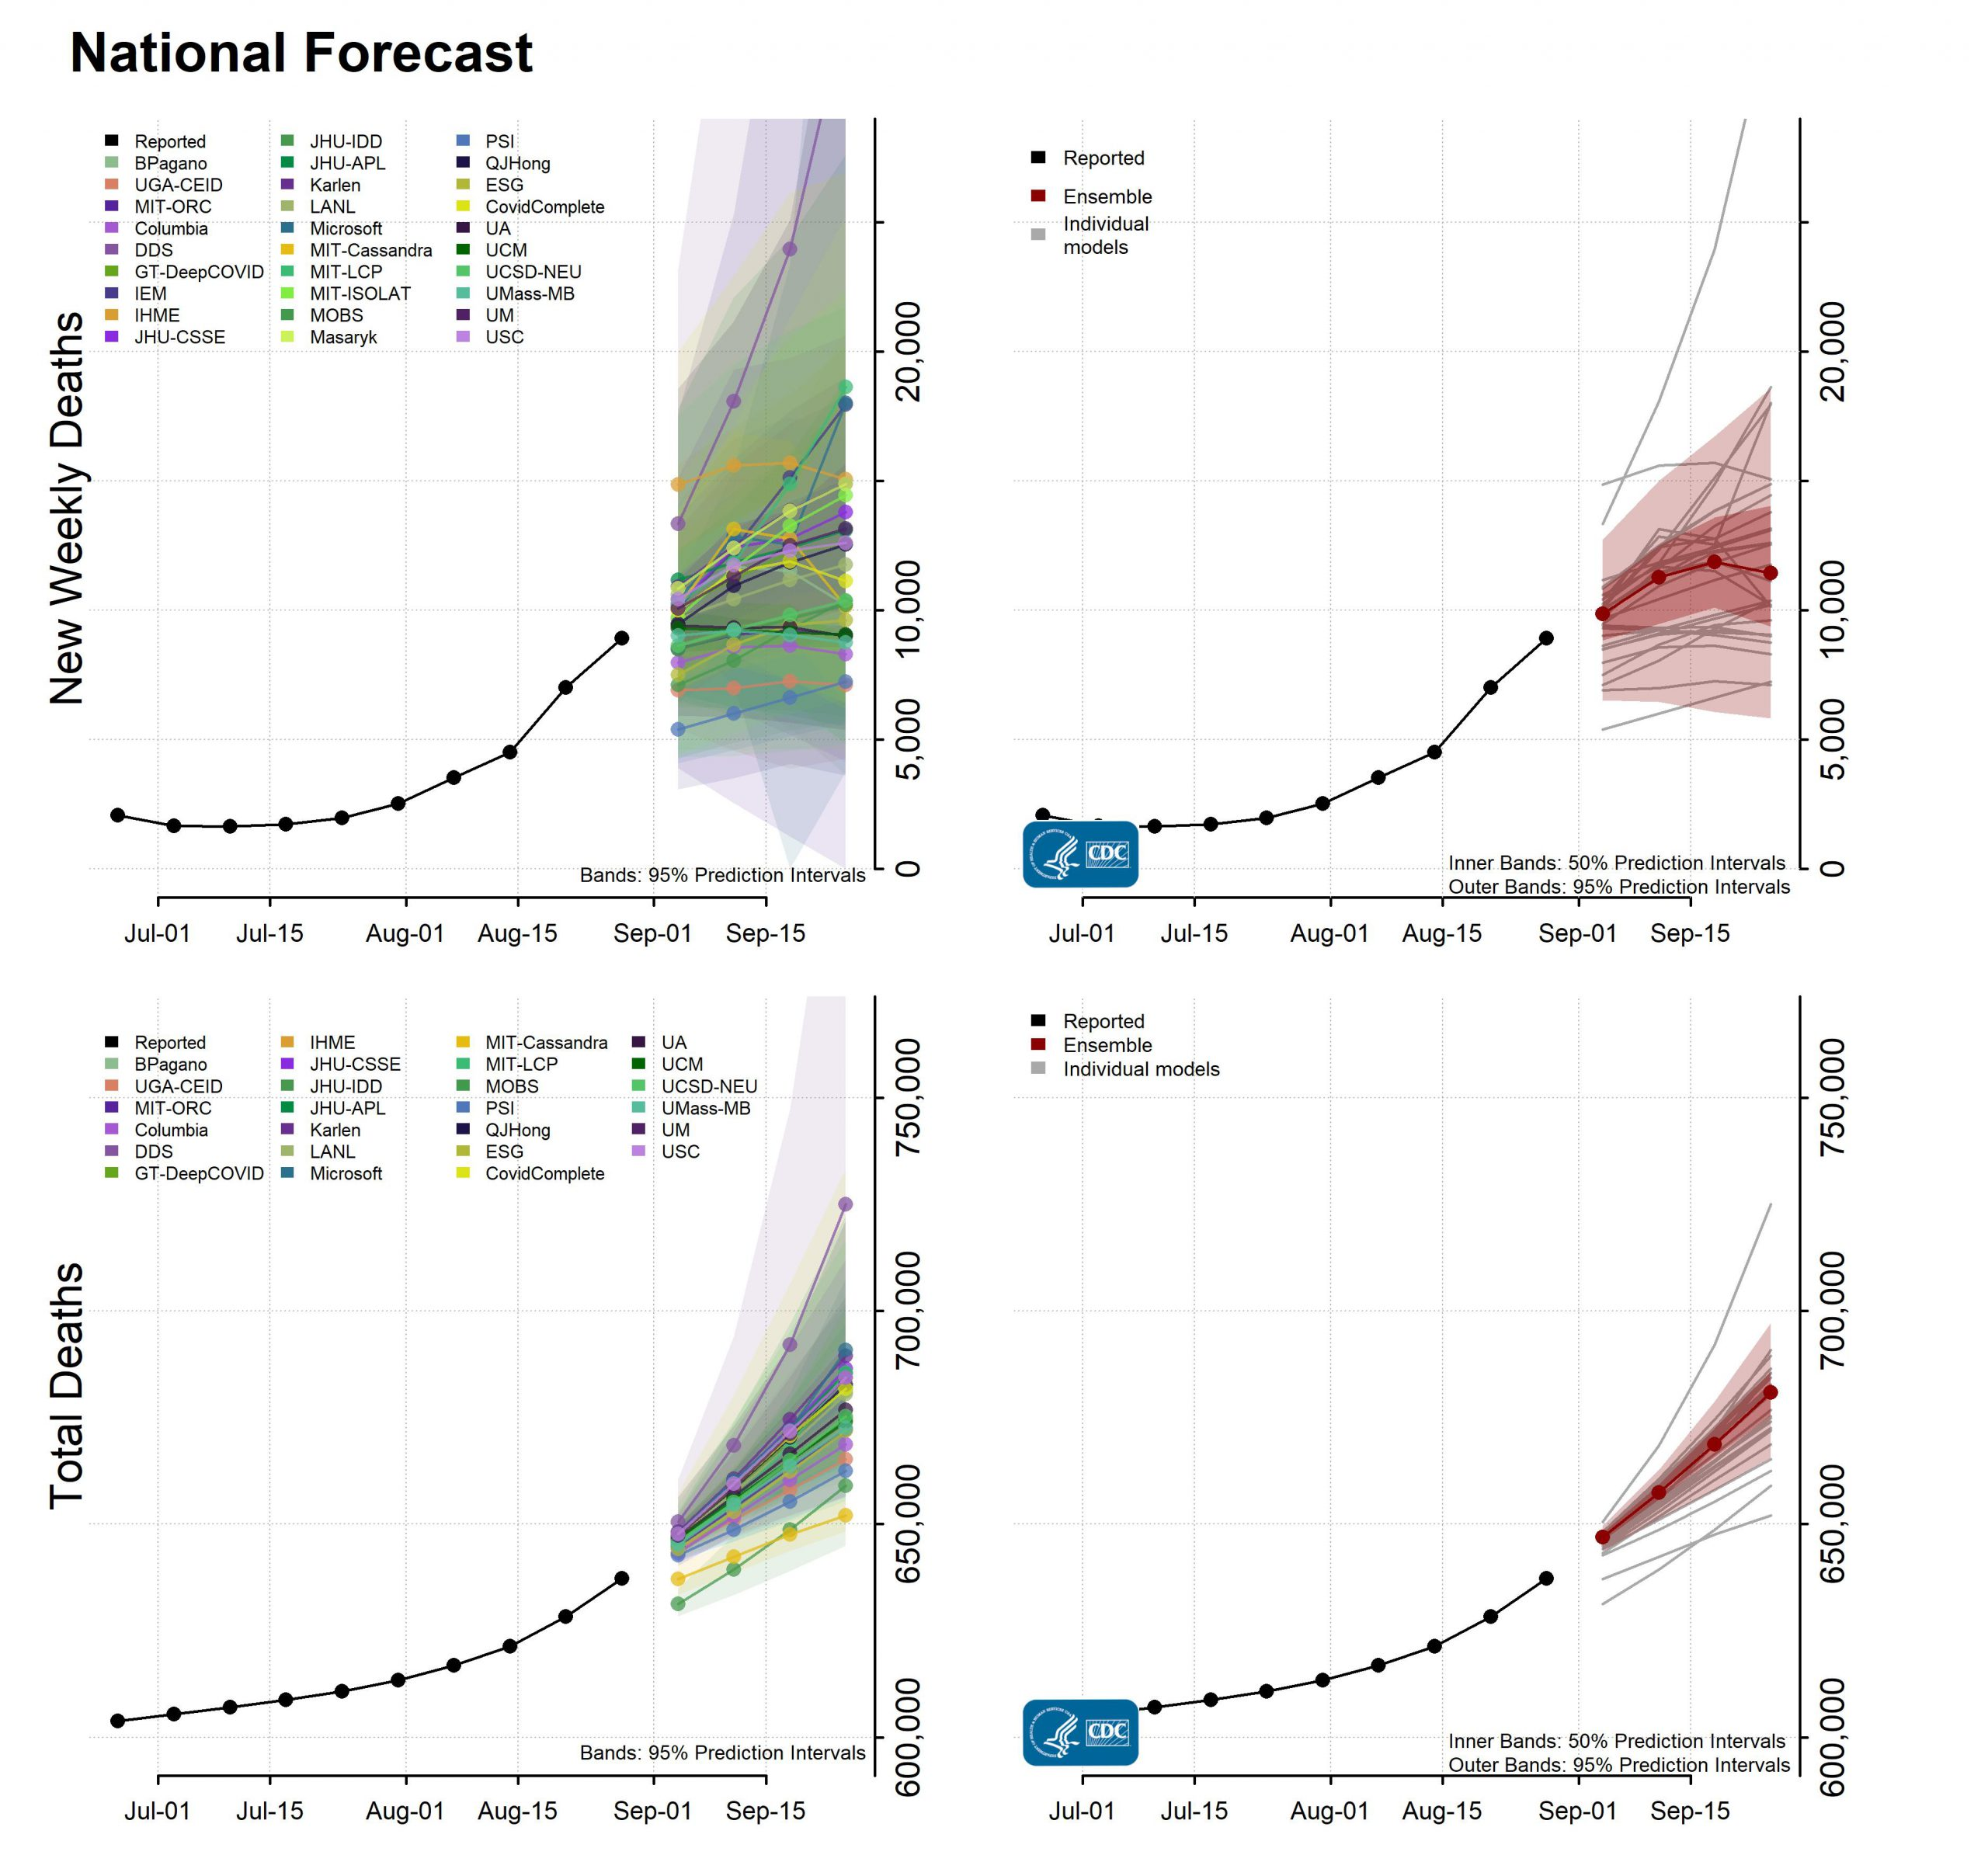
\includegraphics[scale=.12]{Images/8_30_21_cvd_deaths.jpeg}}
\caption[Official CDC COVID-19 deaths report August 2021]{This image, 
published on cdc.gov as official public communication 
by the CDC, shows forecast models for national new weekly deaths due to COVID-19 
in the top row and cumulative deaths on the bottom row. The plots in the left 
column show prediction intervals from multiple teams whereas the plots on the 
right show the intervals for an ensemble forecast model.}
\label{fig:cdcoff}
\end{figure}

\subsection{}
In the context of collaborative forecasting like that of the CDC flu competition
or the COVID-19 Forecast Hub, discretized bins and quantile forecasts have 
proven useful and effective. Yet both types come with their drawbacks. Data 
storage for instance might be a concern if many bins are used for forecasting. 
And scoring methods are limited if forecasts are made of prediction intervals.

In this paper, we propose the use of discrete mixture distributions as a means 
of forecasting for projects similar to the CDC flu competition or the COVID-19
Forecast Hub. In section \ref{section:representations}, 
popular probabilistic forecast representation 
types are defined and reviewed. Methods of scoring, storing, building 
ensembles and other aspects will be reviewed and compared for each 
representation type.
In section \ref{section:conmixforc}, details for using discrete mixture 
distributions in a collaborative forecast project are presented as well as tools
which may be used for scoring and ensemble building.
Section \ref{section:retrostud} is a retrospective study of the CDC flu 
competition and COVID-19 
forecast predictions and an attempt to assess whether any predictions 
approximately come from well known continuous distributions. This paper is 
concluded with a discussion.






















\section{Probabilistic Forecast Representations}
\label{section:representations}

Before introducing discrete mixture distributions as a representation type for a
probabilistic forecast, we review representations already commonplace in 
forecasting. In a collaborative setting, certain aspects of each representation
should be considered. With each representation presented, 
commmon applications of 
scoring, data storage and ensemble construction will be considered for
as well as other notable properties.

\subsection{Representation properties to consider in collaborative projects}
\subsubsection{Scoring}
Scoring rules are used to numerically evaluate or score a probability forecast. 
The
score is a measure of the accuracy of the forecast and where multiple forecasts
exist the score for each may be used to compare forecasts. If a scoring rule 
is proper, then the best possible score is obtained by reporting the true 
distribution. The rule is strictly proper if that value is unique. 
Under proper
scoring rules, a forecaster has no incentive to be dishonest in their 
submission \cite{gneiting2007strictly}. This makes proper scoring rules ideal
for evaluating forecasts. We will limit our review of scoring methods to rules
which are proper.

\subsubsection{Storage}
For a collaborative forecast project where many researchers are involved and 
many predictions are collected, computer storage may need to be addressed. 
As an example of required computer storage, the 
repository for the
COVID-19 Forecast Hub predictions contained 85 million predictions as of 
February 5, 2022 which required more than 11.6 gigabytes of storage!
(cite zoltar??)
When determining the goals of a forecast project, there should be consideration 
of the storage required for different forecast representation types.

\subsubsection{Ensemble Modeling}
A multi-model ensemble is a statistical model made by combining information from
two or more individual statistical models. Private and public decisions are 
regularly made after combining information from multiple sources. For any given
situation, information from one source may provide insight on a subject which 
other
sources fail to capture. Likewise one statistical model may provide insight
that another model does not, so that when they are combined in an ensemble the 
ensemble model outperforms the individual component models.

As probabilistic forecasting becomes more commonplace, so too does ensemble 
modeling. Multi-model ensembles have been used extensively in weather and
climate modeling \cite[for example]{baran2018combining}, 
and they have been used increasingly in modeling infectious disease outbreaks
see \cite[for example]{yamana2016superensemble}. 
Multi-model ensembles allow for an incorporation of multiple signals -
often from differing data sources- and sometimes individual model biases are 
canceled
out or reduced by biases in others \cite[see references
therein]{reich2019accuracy}. 
In several disease outbreak studies, multi-model ensemble forecasts have been 
shown to outperform individual model forecasts 
\cite[see
references therein]{cramer2021evaluation}.

Construction of an ensemble may be done by combining individual forecast 
distributions using weighted averages. This has been called stacking 
\cite{wolpert1992stacked} or weighted density ensembles 
\cite{ray2018prediction}. 

\subsection{Probabilistic Forecast Representation Types}
\subsubsection{Parametric distributions}
\label{section:pardist}
A parametric distribution is a discrete or continuous probability distribution 
described by a known function $p(x) := p(x|\theta)$ -pmf in the discrete case or 
pdf in the continuous case. Here $\theta$ is a vector of known or unkown 
parameters 
contained in a parameter space. 

The value of $p(\cdot)$ evaluated at $x$ is defined as 
$p(x) = P(X = x)$ or the probability that the random variable $X$ takes
on $x$ in the space of the random variable. In the continuous case 
$P(X = x) = 0$ for all $x$, but the probability 
that $X$ falls within an interval $(a,b)$ is calculated as

\begin{equation}
\label{eq:prob}
  P(a < X < b) = \int_a^b p(x) dx
\end{equation}

Other functions classified by a parameteric distribution include the cumulative
distribution function (CDF) and the inverse CDF or quantile function. The CDF 
in the continuous case is defined as

\begin{equation}
\label{eq:ccdf}
  F(x) = P(X \leq b) = \int_{-\infty}^x p(t) dt
\end{equation}
or in the discrete case 

\begin{equation}
\label{eq:dcdf}
  F(x) = P(X \leq b) = \sum_{k=1}^n p(x_k) dt
\end{equation}
where $x_n$ is the largest value of X less than or equal to $x$.
The quantile function is defined as
\begin{equation}
\label{eq:quant}
  Q(p) = \inf \{ y \in \mathbb{R} : p \leq F(x) \}
\end{equation}
returning a quantile value where $p$ is a given probability $0\leq p \leq 1$.

% \subsubsubsection{Scoring}
For a forecast represented as a parametric function with pmf/pdf $p_m(x)$, 
the accuracy of the forecast may be measured as how likely realized value $x^*$
is to occur. Commonly used proper scoring rules for parametric distributions
include the Logarithmic score (LogS), 
continuous rank probability score (CRPS) \cite{hersbach2000decomposition}
\cite{alves2013ncep} and the interval/Brier 
score (IS) \cite{gneiting2007strictly} among 
others. See also \cite{gneiting2014probabilistic}
section 3 for more on proper scoring functions. Unless otherwise noted, the 
following
definitions can be found in the review by Krueger.

For a forecast with pdf/pmf $p_m(x)$, the LogS evaluates the 
probability of the observed value $x^*$. It is defined as

\begin{equation}
\label{eq:logs}
  LS(p_m,x*) = -log\;p_m(x^*)
\end{equation}
The goal is to minimize the LogS, so a forecast $p^{'}_m(x^*)$ is considered 
superior to $p_m(x^*)$ if
$LS(p^{'}_m, x^*) < LS(p_m, x^*)$.
The LogS is limited to scoring forecasts with density functions and
evaluating those densities only at the point $x^*$.

The CRPS is a function of a CDF $F$
and so it may
be used more extensively than the LogS. 
For the CDF $F_m$, the CRPS is defined as

\begin{equation}
\label{eq:crps}
  CRPS(F_m, x^*) = \int_{-\infty}^{\infty} (F_m(x)- 1_{\{x*\leq x\}})^2 dy
\end{equation}
Here too a smaller score indicates a better forecast.

Besides evaluating forecasts, the CRPS may also be used for optimizing weights 
used
to build ensembles under Bayesian model averaging (BMA). Considered the 
state-of-the-art techniques for combining 
component distributions
into a multi-model ensemble are nonhomogeneous regression (NR), also known as
ensemble model output statistics (EMOS), and ensemble
BMA, both of which are defined in \cite{gneiting2014probabilistic}.

In the context of an ensemble made from component models submitted from various
sources,
BMA is the better option. In BMA, the final model does not have to be specified
beforehand and the resulting forecast will be a discrete mixture distribution
of all component forecasts. The general form for an ensemble distribution $p^E$
is

\begin{equation}
\label{eq:bma}
  p^E(x) = \sum_{m=1}^M w_mp_m(x)
\end{equation}
where $p_m$ is the $m^{th}$ component forecast distribution and 
$0 \leq w_m \leq 1$ is a weight assigned to that component where $\sum w_m = 1$.
Methods for estimating weights include Maximum Likelihood estimation
\cite{raftery2005using}, MCMC 
sampling see \cite{vrugt2008ensemble}
and minimizing the ensemble CRPS see
\cite{baran2018combining}.

For selecting distribution weights, the CRPS has some nice properties, but can 
sometimes be
difficult to compute. For example, when the forecast is a mixture of a 
truncated normal distribution (TN) and a truncated lognormal (TL) the CRPS is 
not available in closed form \cite{baran2018combining}.

Generally computation and evaluation of parametric distributions is not hard. 
For most commonly used parametric distributions -normal, lognormal, Poisson,
gamma, etc.- there is software readily available to compute density, 
distribution and quantile values. Likewise, requirements for storage are low 
compared to other representation types that will be discussed. The most common
parametric distributions can be fully defined with three or pieces of data
including
the distribution family and two or three parameters. Table \ref{table:pstor} 
contains
enough information to completely define a $Lognormal(1,0.4)$ distribution.

\begin{table}[h!]

\centering
 \begin{tabular}{|c c c|} 
 \hline
 family & param1 & param2 \\ [0.5ex] 
 \hline
 lnorm & 1 & 0.4 \\ 
 \hline
 \end{tabular}
 \caption[Parametric distribution storage]{Storage example of parametric 
 lognormal 
 distribution with 
 parameters $\mu = $ 1 and $\sigma =$ 0.4}
 \label{table:pstor}
\end{table}

A completely defined continuous parametric distribution can be evaluated at an
infinite number of values. We will call this an infinite resolution.


A drawback of representing a forecast in a parametric distribution is the lack 
of flexibility in the model selection. Easy computation and evaluation of these 
models is limited to what is available in software, so certain distributional
shapes may unattainable. The distribution may also assign probability to values
outside the range of the forecast. There are remedies for this such as 
truncation, but these increase the complexity in evaluation and scoring.
Requiring a parametric forecast also bars the use of some statistical methods
which might be used to create a forecast model including some Bayesian methods
where a posterior distribution cannot be computed in closed form.


\subsubsection{Sample Distributions}
Some forecast model builders may want more flexibility in modeling than a 
parametric 
distribution can provide. Methods that require sampling from a posterior 
distribution or Bootstrap sampling to obtain a sample distribution are examples
where parametric distributions may not be appropriate for modeling.

A sample distribution is made of a sample of random variables 
$(X_1,...,X_n)$ where $X_i \sim D$ and $D$ is a distribution. From this, sample
statistics such as mean, median, variance and quantiles may be calculated. 
An empirical cumulative distribution function (ECDF) may also be calculated as

\begin{equation}
\label{eq:ecdf}
  F_n(x) = \frac{1}{n} \sum_{i=1}^n \mathbb{I}(X_i \leq x)
\end{equation}

According to the Strong Law of Large numbers, the sample mean will converge to
the expected value of the distribution as $n \rightarrow \infty$ as long as the 
expected value of that distribution exists. Likewise by the same law the 
ECDF will converge to the true CDF 
as $n \rightarrow \infty$. Thus, if a sufficiently large 
sample is generated from a distribution with an expectation, 
the sample will closely approximate the 
true distribution. 

For common distribution families it is easy to generate large samples using 
existing functions in \texttt{R} and other programming platforms. For some 
distributions 
for which the mathematical formula is unkown or is not in closed form, more 
sophisticated methods may be required to generate samples. Bayesian analyses may 
require a Gibbs or Metropolis-Hastings algorithm, among others, to generate a 
sample. Such samples are useful in that the true distribution may be closely 
approximated without knowing the true mathematical form. 

Under the samle distribution format, the options that a researcher has for 
constructing a forecast are more than
if they are asked to submit a parametric distribution and the range 
characterisitcs 
and shapes of distributions is larger.
In the last few decades, increased computing power and improvements in MCMC
sampling have greatly contributed to growth in the use of
predictive distributions \cite{gneiting2007strictly}
\cite[see examples listed therein]{krueger2016probabilistic}.

To properly score a forecast represented by a sample distribution, both the CRPS
and LogS may be used. The CRPS has the advantage here of scoring the sample 
distribution directly since the CDF in  (\ref{eq:crps}) may be replaced by the 
ECDF in
(\ref{eq:ecdf}). To use the LogS to score a forecast, a density function for the 
sample must be approximated. Common approximations include a kernel density (KD)
or Gaussian approximation (GA).

KD is defined by Krueger et. al as

\begin{equation}
\label{eq:kd}
  \hat{p}_n(x) = \frac{1}{n h_n} \sum_{i=1}^n K \left( \frac{x-X_i}{h_n} \right) 
\end{equation}
where $K$ is a kernel function, and $h_n$ is a suitable bandwidth. GA is defined
as 

\begin{equation}
\label{eq:ga}
  \hat{F}_n(x) = \Phi  \left( \frac{x-\hat{\mu}_n}{\hat{\sigma}_n} \right)
\end{equation}
where $\Phi$ is the standard normal CDF and $\hat{\mu}_n$ and $\hat{\sigma}_n$
are the empirical mean and standard deviation of the sample $(X_i)$
\cite{krueger2016probabilistic}.

Krueger et. al compare scoring of MCMC drawn forecast distributions using CRPS 
and LogS over samples directly using ECDF or over density approximations using
KD or GA.

To build an ensemble model from sample distribution forecasts, the BMA 
construction from (\ref{eq:bma}) may be used only replacing $p_m$ with 
$\hat{p}_{n_m}^{KD}$ or $\hat{p}_{n_m}^{GA}$ -approximate KD and GA densities. 
Here as well the optimal weights 
$w_m$ may be estimated by maximizing the likelihood or minimizing CRPS. Then 
the ensemble distribution would take the form of a continuous or discrete
probability mixture distribution. If the desire is that the ensemble still be
a sample distribution, after selecting weights, a sample may be selected by 
randomly selecting a sample from $(X_n)_m$ with probability $w_m$.

A potentially large issue with using sample distributions is the amount of storage
it would require. For example when making MCMC draws from a posterior 
distribution, the final sample distribution can have a sample size of thousands
or tens of thousands. Maybe not all distributions would require such a large 
sample size, but sizes of at least dozens or hundreds would be required for each
forecast prediction. For any project the size of the CDC flu competition or the
COVID-19 Forecast Hub, the storage required would be large and potentially 
expensive.

\subsubsection{Discretized bin distributions}
An alternative to parametric distributions and sample distributions which allows
for higher flexibility in distribution shape than a parametric distribution and 
will usually require less storage space than samples is a discretized bin 
distribution.

A discretized bin probability distribution may be constructed over a set 
$A = [a, b]$ by partitioning $A$ into a set of $K$ bins $\{B_i\}_{i=1}^{K}$
where $B_i = [b_{i-1}, b_i)$ and $\cup_{i=1}^{K} B_i = A$. Based on the problem
to be forecasted, researchers will determine the possible range $A$ and 
select the number of bins and the sizes for each bin. It may be the case
that a collaborative project will set the width of all bins to be equal so that 
$\Delta = b_i - b_{i-1}$ is the same width for all $i$ 
\cite[see for example]{mcgowan2019collaborative}.
To complete the construction, a probability $p_i$ is assigned to each $b_i$ 
where $\sum_{i=1}^{K}p_i = 1$. These probabilities are determined by the 
forecasters. 
This discrete representation with a given bin and assigned probability is in
essence a probability mass function in that the calculation of moments and the 
the cumulative distribution are done the same as for a discrete parametric 
distribution. For a random variable $X$ from a binned distribution to calculate
the $j^{th}$ moment we may use

\begin{equation}
\label{eq:bev}
  EX^j = \sum_{i=1}^n \beta_i^j p_i
\end{equation}
where $\beta_i$ is a value corresponding to bin $B_i$ (such as $\beta_i = b_i$,
$\beta_i = b_{i-1}$ or $\beta_i$ is the mean or mid value in $B_i$). The 
cumulative distribution may be calculated as

\begin{equation}
\label{eq:bcdf}
  P(X \leq b) = \sum_{i=1}^n p_i
\end{equation}
where $p_n$ is the probability for the bin $B_n$ where $b \in B_n$.

If the value to be forecasted takes on discrete values, a common discrete 
distribution, such as a binary or Poisson distribution, may sometimes be used to 
assign probabilities to each of the bins. When the values to be forecasted are
continuous, a forecaster may need to employ a method of discretization to a 
forecast distribution. There are a number of possible ways to do this including
those outlined by Chakraborty and Subrata \cite{chakraborty2015generating}.

The CDC has used a discretized bin distribution representation as the 
format
for their annual influenza forecasting competition and other disease outbreak
forecast projects.
In that context it has become the standard representation 
\cite{brooks2020comparing}. Much work has been done in evaluating 
and constructing ensemble models on influenza forecasts represented by 
discretized bins \cite{mcgowan2019collaborative, mcandrew2019adaptively,reich2019collaborative}. 

Because discretized bins can be seen as a pmf, methods for proper scoring 
already 
discussed -LogS and CRPS- are useable and BMA is valid method for ensemble 
construction. Reich et. al used BMA to combine multiple forecasts from the flu 
competition. They built and compared ensemble models with different weighting
schemes including equally weighted components $w_j = 1/J$ and estimating weights
according to the model specification. To estimate weights they used the 
Expectation Maximization (EM) algorithm 
\cite[see
supplementary material within for details]{reich2019accuracy}.

The exact amount of information required for a discretized bin forecast will 
vary depending on the permitted range of the forecast and the desired 
resolution. 
In the CDC flu contest, a forecast might have 131 bins between 0\% and 13\% 
-bins having increments of 0.1 or 0.001\%- with 
corresponding probabilities in each. This makes 262 pieces of information per
prediction. For any binning scheme of more than two bins, the information 
requirement for discretized bins will be higher than for parametric distrbutions.
Table \ref{table:dbins} illustrates what a discretized 
Lognormal$(1,0.4)$ distribution truncated over $[0,8]$
looks like in 41 equally spaced discretized bins. The discretization was done
such that 

\begin{equation}
\label{eq:disc}
  p_i = \int_{b_{i-1}}^{b_i} p^{TL}(x) dx
\end{equation}
where $p^{TL}$ is the pdf of a truncated Lognormal$(1,0.4)$. This is similar
to Methodology-IV from Chakraborty 
\cite{chakraborty2015generating,kemp2004classes}.

\begin{table}[h!]

\centering
 \begin{tabular}{|c|c|} 
 \hline
    bin & prob \\ \hline
    ... & ... \\
    {[1.4,\;1.6)} & 0.04414 \\
    {[1.6,\;1.8)} & 0.05896 \\
    {[1.8,\;2.0)} & 0.07032 \\
    {[2.0,\;2.2)} & 0.07172 \\
    {[2.2,\;2.4)} & 0.07955 \\
    ... & ... \\
 \hline

 \end{tabular}
  \caption[Discretized bin distribution storage]{Storage example of discretized
  lognormal with $\mu = 1$ and $\sigma = 0.4$}
\label{table:dbins}
\end{table}
Submitted as a forecast prediction, the distribution in table \ref{table:dbins} 
includes 82 pieces of data. For parts 
of the CDC influenza competition some forecasts included up to 262. This is 
far less storage than the possible thousands of draws from a sample 
distribution but is 
still much larger than the three or five data pieces required to report a 
lognormal
or truncated lognormal distribution.

Depending on what is known about the problem to be solved, creating the right 
binning scheme may be a challenge. Because there must be a finite number of
bins, forecast distributions often have a finite support. Where the range of 
possible outcomes to a problem is not well known, the right binning scheme may 
be
hard to produce.









\subsubsection{Quantile representation}
When deciding how forecasts should be represented in the COVID-19 Forecast Hub,
the time pressure of generating forecasts and the consideration of the large
range for possible outcomes both contributed to the COVID-19 Forecast Hub 
decision
to forego trying to create the right binning scheme and use sets of prediction
intervals to represent uncertainty in predictions \cite{bracher2021evaluating}.

The Forecast Hub requires predictions to be submitted as 11 or three nominal 
intervals -depending on the specific target and unit to forecast- and a median.
Using this interval or quantile representation leads to a number of changes in 
the scoring and ensemble building of forecasts.

A quantile forecast is constructed as follows.
For $N$ given quantiles $\alpha_1,..., \alpha_N$; $q_1,..., q_N$ are the values
such that 

\begin{equation}
\label{eq:quantiles}
  P(Y \leq q_1) = \alpha_1, P(Y \leq q_2) = \alpha_2, ..., 
  P(Y \leq q_N) = \alpha_N
\end{equation}
When the quantiles are reported as prediction intervals we have

\begin{equation}
\label{eq:intervals}
  P(Y \leq q_1) = \alpha_1, P(Y \leq q_2) = \alpha_2, ...,
  P(Y \leq q_{N-1}) = 1 - \alpha_2, P(Y \leq q_N) = 1 - \alpha_1
\end{equation}

What is possible for scoring forecasts
or building ensemble models in other representations is often not possible with
quantile forecasts. The shape of a distribution is also not known and in fact,
nothing is known about the tails or the uncertainty beyond the most 
extreme reported quantile values. In the Forecast Hub predictions, nothing 
is reported about the range below the $1^{st}$ quantile or above the $99^{th}$.
Yet the quantile representation has its advantages. 

Quantile representation allows for forecasters to submit fairly detailed
forecasts without restricting the range of possible values.
Since quantiles are easily calculated from any regular distribution type
-e.g. quantile function for parametric functions or calculating sample 
quantiles- we consider quantile forecasts to be highly flexible in terms of 
what methods forecasters may employ in modeling.

To score predictions from a quantile or prediction interval format, 
neither the LogS nor the CRPS may be used, 
but another proper scoring rule the IS may be used.
For an observed outcome $x^*$ and a prediction interval $(l,r)$ 
where $l$ and $r$ are the $\alpha/2$ and $(1-\alpha/2)$ quantiles that bound
the central $(1-\alpha)$ prediction interval the IS is defined as

\begin{equation}
\label{eq:is}
  IS_{\alpha}(l,r; x^*) = (r-l) + \frac{2}{\alpha}(l-x^*)1\{x^*<l\} 
  + \frac{2}{\alpha}(y-r)1\{x^* > r\}
\end{equation}
This is a sum -weighted by 
$\alpha$- of the width of the
interval and the distance between $x^*$ and the interval (if $x^*$ is not 
captured in the interval) \cite{gneiting2014probabilistic}. 
The IS requires only a single central 
$(1-\alpha) \times 100$ prediction interval.

When an interval forecast is made up of multiple intervals each with different
$\alpha$ levels, the weighted interval score (WIS) may be evaluated. Bracher et.
al use the WIS to evaluate COVID-19 inverval forecasts 
\cite{bracher2021evaluating}.
There are multiple versions of the WIS -some of 
which are described in Bracher et. al- but the version used by the COVID-19 
Forecast
Hub for a forecast of $K$ intervals is defined as follows

\begin{equation}
\label{eq:wis}
  WIS_{0,K}(F_m,y^*) = \frac{1}{K + 1/2} \times (w_0, \times |y^*-med|+
  \sum_{k=1}^K \{ w_k \times IS_{\alpha_k}(F_m,y) \} )
\end{equation}
where $w_k = \alpha_k/2$ is the weight on the $k^{th}$
interval. With that choice of weights, it may be shown that the
WIS approximates the CRPS \cite[see S1 Text therein]{bracher2021evaluating}.

Bogner, Liechti and Zappa compared scoring forecasts of quantiles with the 
Quantile Score (QS) similar to the interval score and scoring distribution functions
fit to those quantiles using the CRPS \cite{bogner2017combining}. The CRPS 
corresponds to the integral of the QS over all possible thresholds rather than
just specific quantiles, so it more effectively reveals deficiencies in parts of 
the distribution and especially in the tails past the end points of quantiles
used in QS or IS. Thus there may be something lost in terms of scoring when the 
WIS is used.

Like the CRPS, not only does the WIS provide an easily interpretable proper 
score for interval forecasts, but it may also be useful when building an 
ensemble forecast.
The ensemble forecast constructed by the COVID-19 Forecast Hub was made as an
equally-weighted average of forecasts from the component models. More 
specifically, each quantile value of the ensemble was the average of values from
all models corresponding to the same quantile \cite{ray2020ensemble}. For $M$ 
models each with $K$ quantiles, the $k^{th}$ ensemble quantile $q^E_k$ is 
calculated as

\begin{equation}
\label{eq:qa}
  q^E_k = \sum_{m=1}^M \nu_m q_k^m 
\end{equation}
where $\nu_m$ is the weight assigned to each forecast and $\sum \nu_m = 1$. In
the Forecast Hub model, $\nu_m = \nu = 1/M$. Where the overall mean or a
weighted mean may be used, the median may also be used.
Brooks et. al compare performance of the COVID-19 ensemble
between equally-weighted means, weighted means and median value constructions.
\cite{brooks2020comparing} (is is appropriate to cite this blog??)
In their report, they show that weighted means and median constructions tend
to outperform an equally-weighted mean construction. To come up with optimal 
weights, they select values $\nu_m$ from (\ref{eq:qa}) which minimize the WIS of 
the ensemble forecast.

Averaging quantiles in this way is the same as quantile averaging or Vincentization
only with an incomplete quantile function. It thus carries with it many of the
same characteristics.
Quantile averaging or Vincentization for a complete distribution is defined as 

\begin{equation}
\label{eq:vinc}
  F_v^{-1}(\alpha) = \sum_{m=i}^M w_m F_m^{-1} (\alpha)
\end{equation}
where $F_m^{-1} (\alpha) = \inf \{y:F_m(y) \geq \alpha\}$ for 
$0 < \alpha \leq 1$. Some notable characteristics are that it is more likely for
the ensemble distribution
to be unimodal than it is under linear averaging of densities like BMA 
\cite{busetti2017quantile} Under some circumstances, such as when member
distributions are exponential, Weibull or logisitic the aggregated distribution
is the same \cite{ratcliff1979group}. It produces smoother
distributions than BMA according to Schepen and Wang \cite{schepen2015model}.
Lichtendahl et. al conclude that quantile averaging produces sharper forecasts
and tends to perform better in scoring than probability averaging
\cite{lichtendahl2013better}.

As in sample distributions and binned distributions, 
data storage for interval forecasts will
depend on the desired clarity of resolution. For the COVID-19 forecasts 
submitted to the Forecast Hub, 23 quantile values are requested for 
the quantiles (0.01, 0.025, 0.05, 0.10, …, 0.95, 0.975, 0.99). This included a 
median along with eleven confidence intervals \cite{bracher2021evaluating}. This
requires forecasters to submit 46 values in each short-term forecast 
(some of the longer term forecasts only include seven quantiles). In terms of 
storage, this is an improvement over requirements for the flu contest. Table
\ref{table:qstor} shows what a submission of 23 quantiles from a 
$Lognormal(1,0.4)$ looks like.



\begin{table}[h!]
\centering

 \begin{tabular}{|c||c|c|c|c|c|c|c|c|c|}
 \hline
    quantile & 0.01 & 0.025 & 0.05  & ...  & 0.95 & 0.975 & 0.99 \\ \hline
    value & 1.07137 & 1.2404 & 1.40689 & ... & 5.18328 &
    5.82391 & 6.58783 \\
    
 \hline
 \end{tabular}
 \caption[Quantile/interval and values storage]{Storage example of quantiles 
 and values of lognormal with $\mu = 1$ and $\sigma = 0.4$}
 \label{table:qstor}
\end{table}



\begin{figure}[htbp]
\centerline{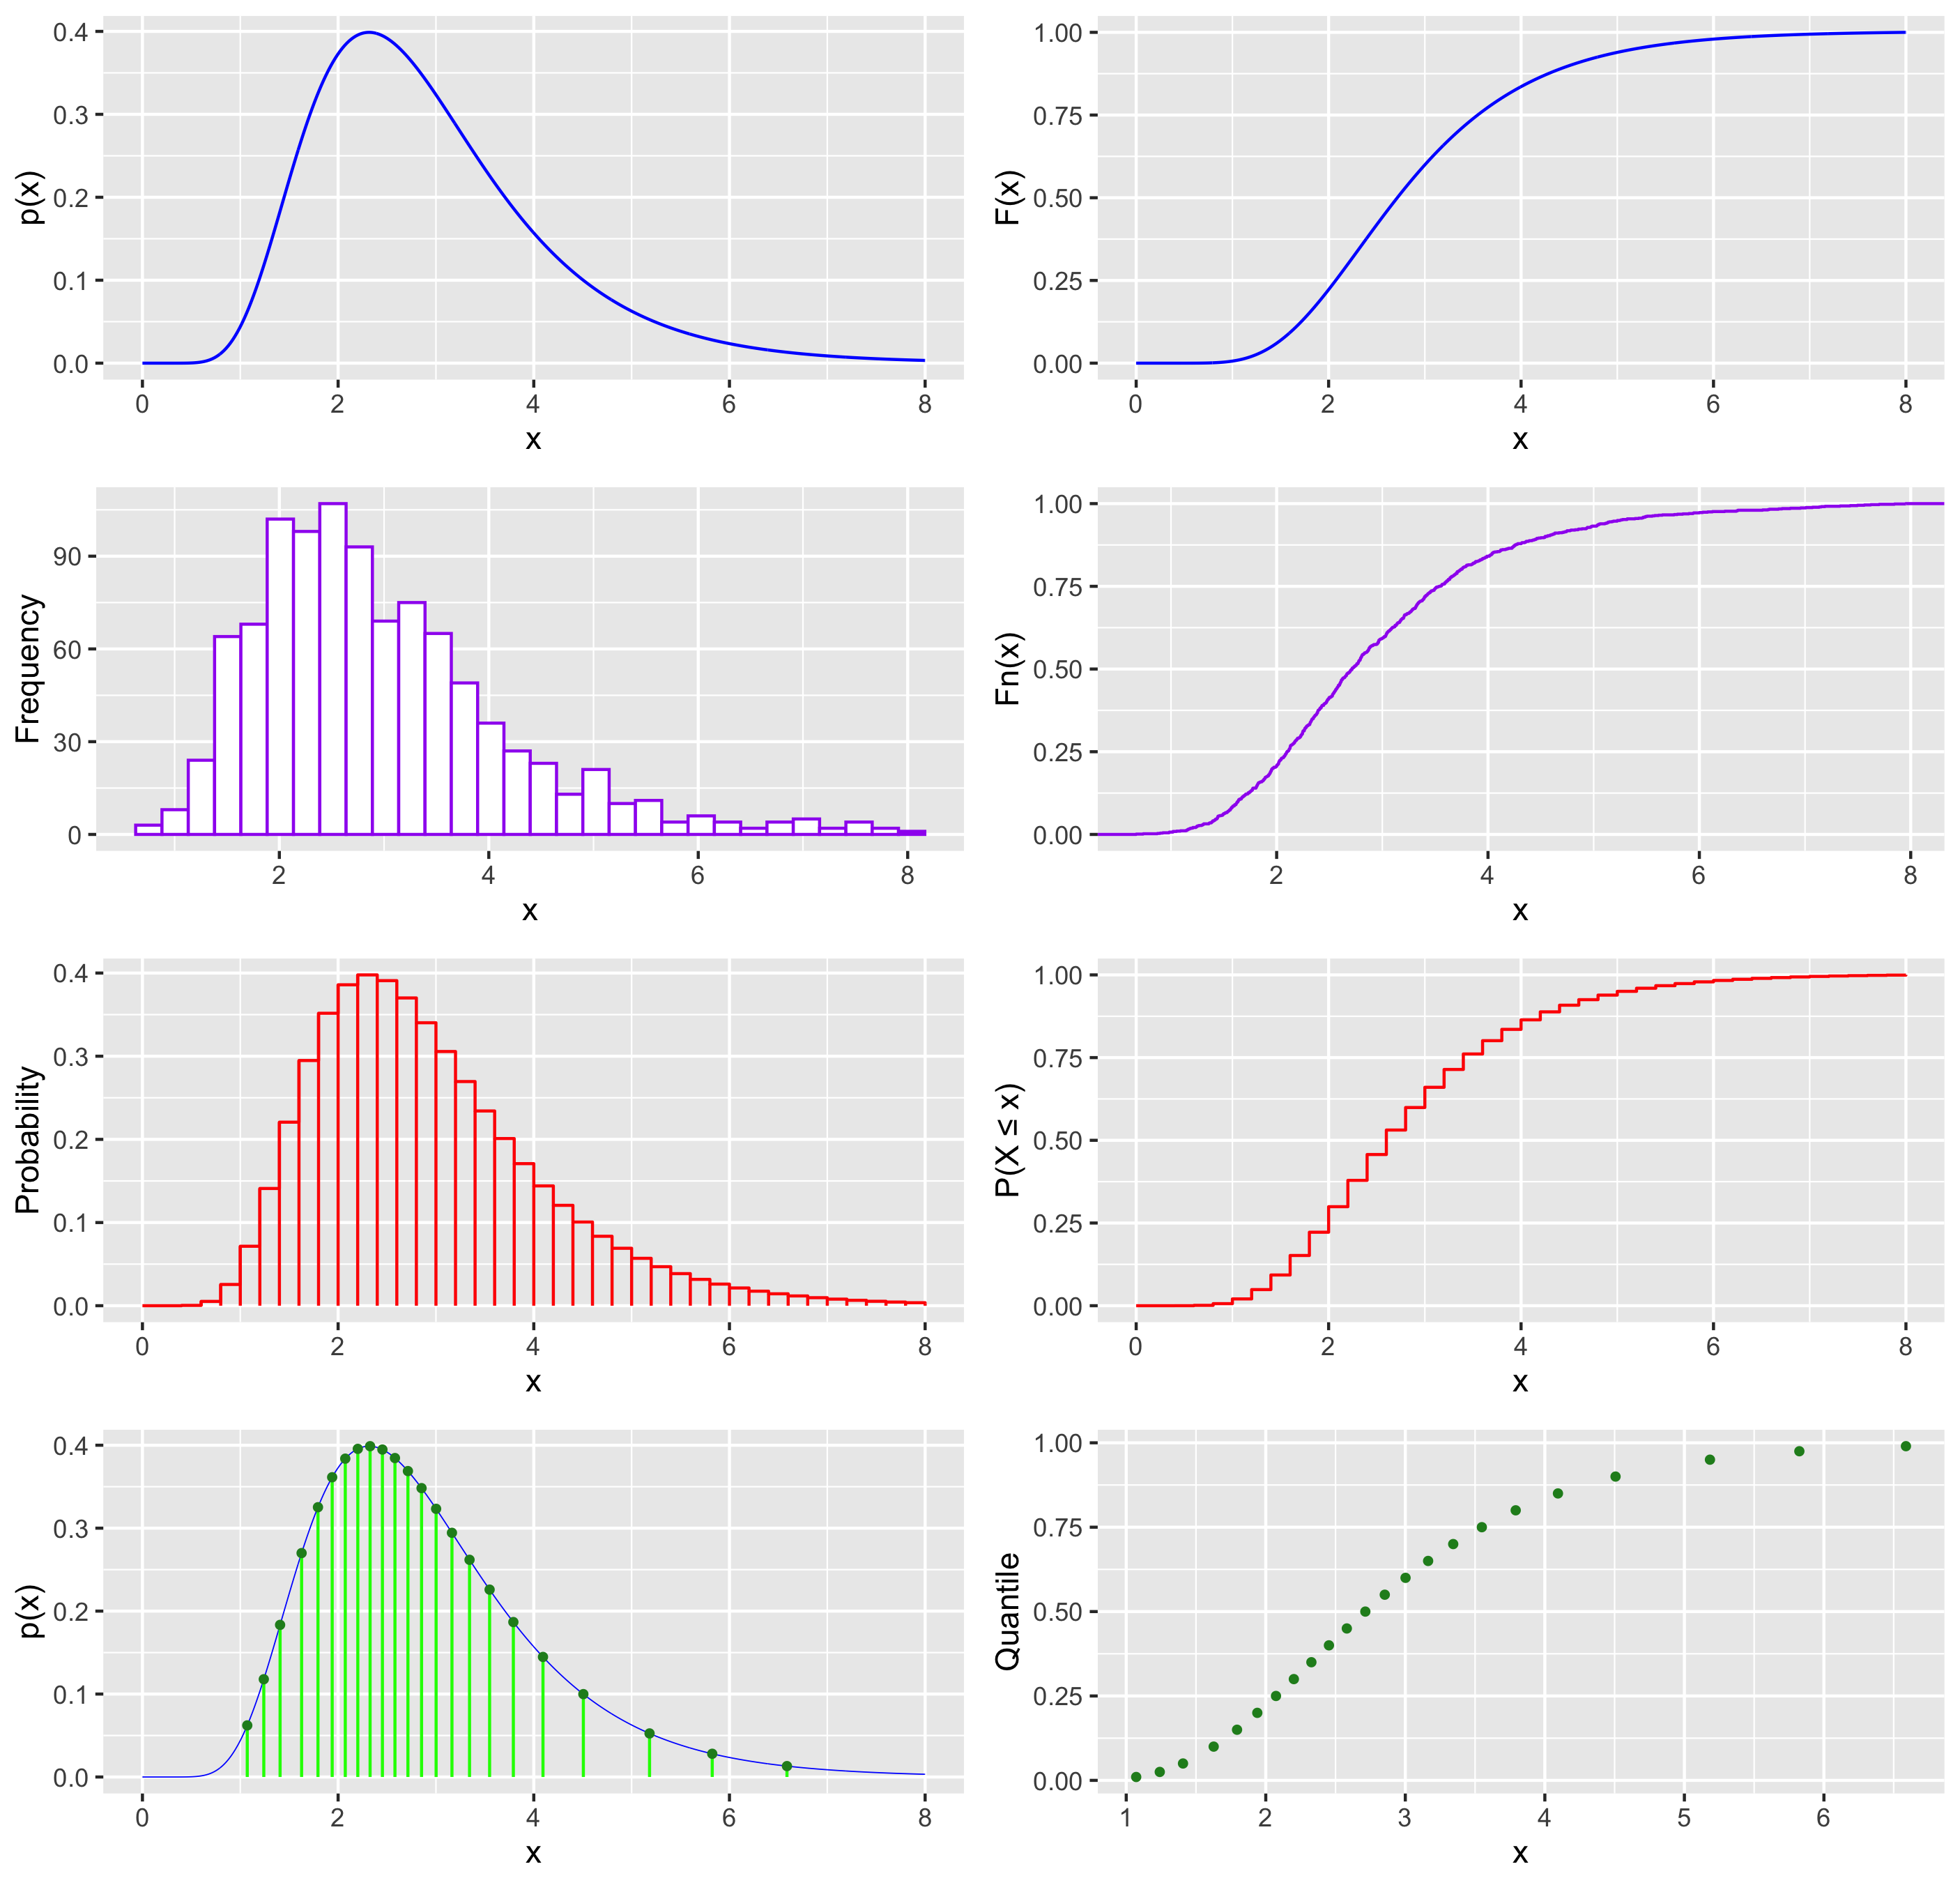
\includegraphics[scale=.1]{Images/dens_cum_comp.png}}
\caption[Density/CDF comparison between parametric distribution, sample 
distribution, discretized bin distribution and quantiles]{This figure compares 
the
densities and CDFs of forecast representation types discussed in the left and 
right columns respectively. Each is generated from a lognorma(1,0.4) 
distribution. Blue shows the density and CDF functions. Purple shows a 
histogram and ECDF of 1,000 samples. Red shows bin probabilities and the CDF
function. Green shows quantiles/intervals with corresponding values.}
\label{fig:denscomp}
\end{figure}




\subsection{Discrete mixture of parametric distributions}
A discrete mixture of parametric distributions forecast representation may be an
attractive alternative to the four types already discussed. A discrete mixture 
would allow for many distribution shapes, a high resolution, storage comparable
to that of discretized bins and quantile representations and the use of the more
common methods for scoring and ensemble building.

A discrete mixture distribution may be constructed in the same way as the
ensemble described in section \ref{section:pardist} in equation 
(\ref{eq:bma}) 
where for $T$ distributions
with pdfs $p_t(x)$ and $z_t > 0$ and $\sum_{t=1}^{T} z_t = 1$
 

\begin{equation}
\label{eq:dmd}
  p^{M} = \sum_{t=1}^T z_tp_t(x)
\end{equation}




Like the standard parametric model, a discrete mixture may be evaluated with
exisiting software (like distr \texttt{R} package \cite{camphausen2007distr}). 
And 
scoring may be done by 
using the LogS, CRPS and IS. The resolution of a discrete mixture is infinite 
and the support need not be limited by submission requirements. 

A mixture distribution may be much more flexible than a single component 
parametric distribution in 
terms of distributional shape. According to 
McLachlan and Peel, a finite mixture of 
normal densities with common variance can be used to approximate arbitrarily 
well
any continuous distribution \cite{peel2000finite} (see also 
\cite{nguyen2019approximations}). Thus, for an unconventional probability
distribution -such as MCMC posterior samples- it may be reasonable to 
approximate the distribution by constructing a mixture of normals.
% See section \ref{section:conmix} for an example.

An ensemble model may be built by using (\ref{eq:bma}) only replacing $p_m$
with $p_m^M$ in \ref{eq:dmd}. Solving for weights may also be done similarly, 
though with the 
added complexity of component models being mixture distributions the 
computation is likely to be more expensive. An example where this may be
especially true is when minimizing of CRPS, but the exact mixture doesn't 
result in CRPS in closed form \cite{baran2018combining}. In large projects like
the COVID-19 Forecast Hub, if an equal weight is not assigned to each component,
it may be determined that models not reaching a certain standard of predictive
performance are
assigned an ensemble weight of 0. This would simplify an ensemble model to 
include only the best performing forecasts.

Depending on the number of components a forecaster includes in a mixture 
forecast, the amount of storage per forecast might be as little as for a 
parametric forecast and as much as a forecast hub will allow. In section
\ref{section:conmixforc} we show how a mixture distribution may be constructed,
scored and used to construct an ensemble using software available in 
\texttt{R}.

Table \ref{table:repscomp} shows how a discrete mixture distribution forecast 
compares with the other formats discussed in terms of methods for scoring,
information and resolution provided, methods for ensemble building and computer
storage requirement.





\begin{flushleft}
  \begin{table}
    % \begin{adjustwidth}{-3cm}{-1cm}
    \begin{tabular}{ | p{2.4cm} || p{3cm} | p{4cm} | p{3cm} | p{3.5cm} |}
    \hline
    \textbf{Representation} & \textbf{Scoring} & 
    \textbf{Flexibility/Information} & \textbf{Ensemble} &
    \textbf{Storage Requirement}
    \\ \hline \hline

    Parametric & LogS, CRPS, IS & Limited to common distribution families. 
    Infinite resolution
    & BMA & Low 3-6 values per prediction \\ \hline
    
    Samples & CRPS and IS. LogS after smoothing & Any shape. Resolution may be
    very high but depends on sample size & BMA after smoothing. Resampling 
    otherwise & 
    Hundreds or thousands of values per prediction
    \\ \hline
    
    Discretized bins & LogS, CRPS, IS &
    Any shape allowed, but limited by binning scheme. Range also may be limited
    & BMA &
    Depends on binning scheme but dozens to hundreds of values
    \\ \hline


    Quantiles & IS, WIS & Shape unknown but with enough quantiles there is still
    a decent amount of information. No tail information & 
    Quantile averaging & Depends on 
    requested quantiles. Perhaps dozens of values
    \\ \hline
    
    Discrete Mixture & LogS, CRPS, IS. May be more limited by computation & With
    enough component distributions may
    approximate any distribution shape. Infinite resolution& BMA 
    & 3 values to dozens per forecast depending on number of components
    \\ \hline
    
  
   
	 \end{tabular}
	 % \end{adjustwidth}
   \caption[Forecast representation comparison]{This table compares scoring,
   information, ensemble building and storage requirements for the different
   forecast representations discussed.}
   \label{table:repscomp}
   \end{table}
	 
\end{flushleft}



























\section{Mixture distributions in a collaborative forecast project}
\label{section:conmixforc}


The CDC and the COVID-19 Forecast Hub as well as other collaborative projects
have their own established systems for receiving, 
evaluating and constructing ensemble forecasts. A transition from using binned 
distributions or quantile forecasts to using discrete mixture distributions 
nwould require
a few adjustments to those systems. In this section we outline how some of these
adjustments may be implemented as well as present some tools which may be used
to evaluate forecasts and construct ensemble forecasts from multiple models.

\subsection{Submission format}
For a collaborative forecast project to run smoothly, model submissions from all 
modelers should all follow the same format. For both the CDC flu forecasting and
the COVID-19 Forecast Hub, teams are provided a .csv spreadsheet with columns 
similar to those in tables \ref{table:dbins} and \ref{table:qstor}. Additionally
columns for Location, Target, Type and Unit are included which serve as
indicators of the specific prediction. The values for all variables except 
Value come from a specified list from the forecast center. Value is the 
probability assigned to a bin when the Type is Bin.

\begin{table}[h!]
\label{tab:dstan}
\centering
 \begin{tabular}{|c|c|c|c|c|c|}
 \hline
    Location & Target & Type & Unit & Bin & Value  \\ \hline
    US National & Season Onset & Point & week & NA & . \\
    US National & Season Onset & Bin & week & 0.0 & . \\
    US National & Season Onset & Bin & week & 0.1 & . \\
    ... & ... & ... & ... & ... & ... \\
 \hline
 \end{tabular}
 \caption[Influenza competition submission example]{Example of a submission file
 for an discretized forecast like those in the CDC influenza forecast 
 competition. To match a quantile submission format as used by
 the COVID-19 Forecast Hub, possible values for the variable Type are Point and
 Quantile, the Bin column is replaced with a Quantile column and Value is 
 the value of the specified quantile in the forecast.}
 \label{table:dstan}
\end{table}

For the quantile forecasts of the Forecast Hub, the main changes to table
\ref{tab:dstan} are that the possible values for Type 
are Point and Quantile, and rather than using a Bin variable Quantile is used
with values specified by the Hub. Then Value rather than a probability is the
forecasted value for the specified quantile. Per prediction there may be a 
couple dozen rows, up to 24 in the Forecast Hub, or over 100 rows as in some
flu forecasts. 

In the discrete mixture format, an adjustment may be made to the format of table 
\ref{table:dstan} where each 
row
represents a component in a mixture distribution.
The variables Bin/Quantile and Value are removed and replaced with Family,
Param1, Param2 and Weight where Family is the distribution family,
Params are the parameters for the component distribution and Weight is the 
weight $w_i$ for that component.

\begin{table}[h!]
\centering
 \begin{tabular}{|c|c|c|c|c|c|c|c|c|}
 \hline
    Location & Target & Type & Unit & Family & Param1 & Param2 & Weight
    \\ \hline
    US National & Season Onset & Dist & week & norm & $\mu_n$ & $\sigma_n$ & .\\
    US National & Season Onset & Dist & week & lnorm & $\mu_l$ & $\sigma_l$ &.\\
    ... & ... & ... & ... & ... & ... & ... & .\\
 \hline
 \end{tabular}
 \caption[Mixture distribution forecast submission example]{Example of a 
 submission file
 for a disease outbreak forecast using mixture distribution representation}
 \label{table:dstan}
\end{table}

A forecast center may want to limit the number of components allowed per 
prediction. For reference, a mixture distribution prediction following the 
format in table \ref{table:dstan} with 18 
components would require $18 \times 8 = 144$ cells submitted. This is the same 
number of cells
submitted for a Forecast Hub forecast with 23 quantiles and a point prediction 
according to the format in table \ref{table:dstan}.

Throughout the remainder of this section, explanations of how to work with 
mixture distributions along with \texttt{R} code which will be given to 
demonstrate constructing a mixture distribution from a forecast submission, 
scoring the forecast and building an ensemble forecast.

\subsection{Mixture construction and scoring tools}
\label{section:tools}

From a submitted forecast, a prediction may be found by Location, Target and 
Unit (or whatever other indication variables are used by collaborators) and 
evaluated. We found
the \texttt{distr} package \cite{camphausen2007distr}
useful for constructing a mixture distribution given
information like that from table \ref{table:dstan}. 

The function 
\texttt{UnivarMixingDistribution} takes as arguments a list of distributions
and a vector of weights for each distribution and a object of class 
\texttt{AbscontDistribution} is returned. The object is in essence a mixture
distribution of the form of (\ref{eq:dmd}). Functions for density, 
distribution
and quantile functions as well as for random sampling may then be used on the
mixture distribution object for evaluation. Using those functions and the 
created object, LogS and CRPS are easily calculable. 

We wrote a function \texttt{MakeDist} (see Appendix)
which takes on a data frame with variables
Family, Param1, Param2, Param3 and Weight and returns a mixture distribution 
of component distributions specified in the rows.

Beginning with two forecast submissions of the form of table \ref{table:dstan}, 
say we select from each a prediction of an event for the same location, target
and unit. The following two data frames \texttt{preddf1} and \texttt{preddf2}
are the resulting predictions.

\begin{table}[h!]
\centering
 \begin{tabular}{|c|c|c|c|c|}
 \hline
    family & param1 & param2 & param3 & weight
    \\ \hline
    Lnorm & 2 & 1 & NA & 0.3  \\
    Norm & 2.1 & 1 & NA & 0.7 \\
 \hline
 \end{tabular}
 \caption[Toy prediction 1]{Toy prediction 1}
 \label{tab:preddf1}
\end{table}

\begin{table}[h!]
\centering
 \begin{tabular}{|c|c|c|c|c|}
 \hline
    family & param1 & param2 & param3 & weight
    \\ \hline
    Norm & 1.5 & 1 & NA & 0.4  \\
    Norm & 4 & 2 & NA & 0.6 \\
 \hline
 \end{tabular}
 \caption[Toy prediction 2]{Toy prediction 2}
 \label{tab:preddf2}
\end{table}

The code here shows these two data frames and how the \texttt{MakeDist} 
function is used to create the distributions in \texttt{R}. Once the 
distributions are created as \texttt{AbscontDistribution} classes, then 
functions for evaluating a pdf and a CDF for each are created.


\begin{Schunk}
\begin{Sinput}
> preddf1
> #  family param1 param2 param3 weights
> #1  Lnorm    2.0      1     NA     0.3
> #2   Norm    2.1      1     NA     0.7
> 
> preddf2
> #  family param1 param2 param3 weights
> #1   Norm    1.5      1     NA     0.4
> #2   Norm    4.0      2     NA     0.6
> 
> 
> 
> #make mixture distributions from prediction submissions
> mdist1 <- MakeDist(preddf1)
> mdist2 <- MakeDist(preddf2)
> #make pdfs for mixture predictions
> dmdist1 <- function(x) {distr::d(mdist1)(x)}
> dmdist2 <- function(x) {distr::d(mdist2)(x)}
> #make cdfs for mixture predictions
> pmdist1 <- function(x) {distr::p(mdist1)(x)}
> pmdist2 <- function(x) {distr::p(mdist2)(x)}
\end{Sinput}
\end{Schunk}

\begin{figure}[htbp]
\centerline{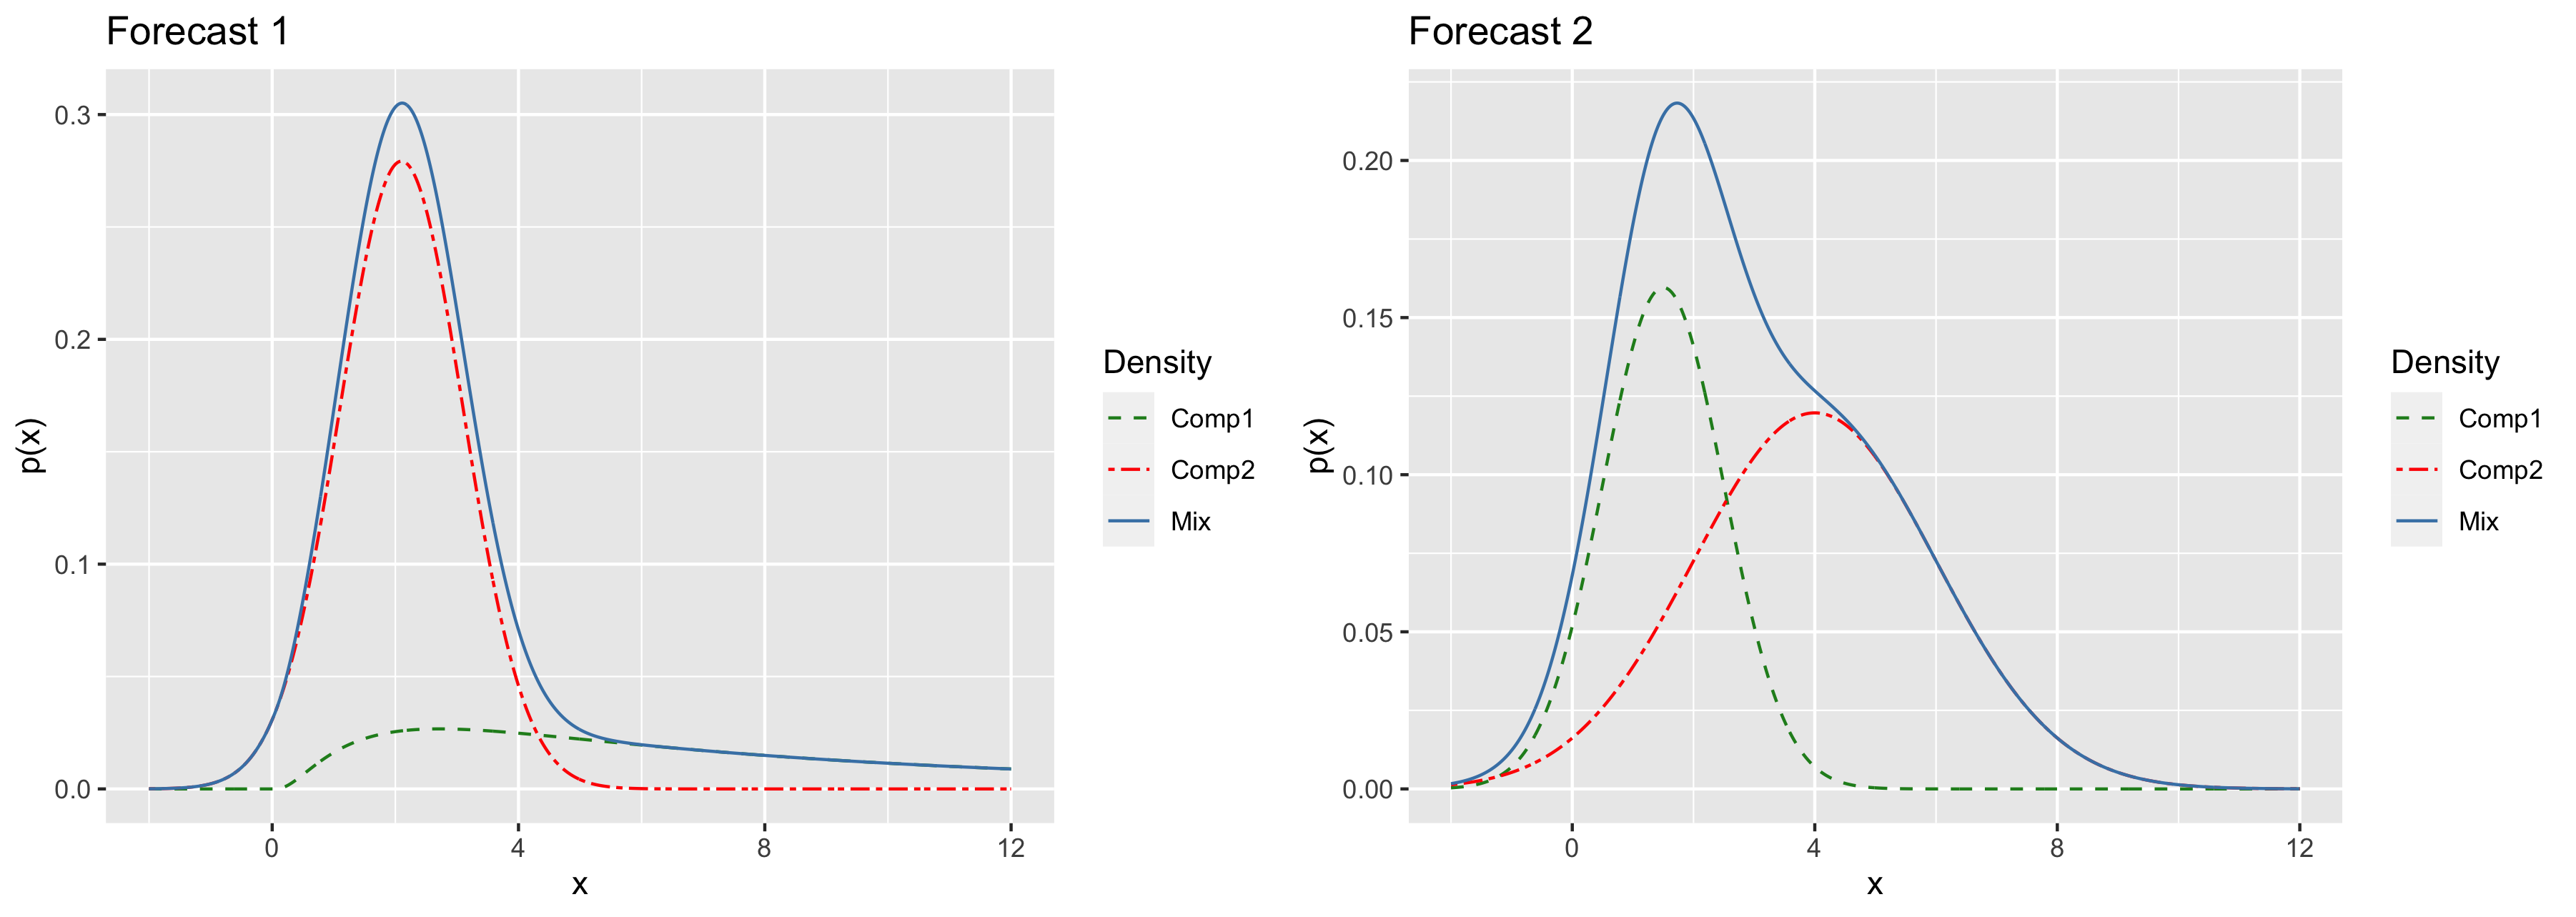
\includegraphics[scale=.15]{Images/toyfors12.png}}
\caption[Toy mixture distributions]{These plots show the density functions of
the two toy mixture distribution forecasts along with the component density
functions scaled by the corresponding weights}
\label{fig:toymixs}
\end{figure}


The LogS or the CRPS may then be calculated for each forecast using the pdf
and cdf functions respectively. Here will will assume that the realized value
which both forecasts attempted to predict was 3. The \texttt{CRPS()} function 
here is 
included in the appendix of this manuscript. It can be seen here that by the 
LogS, the forecast from table \ref{tab:preddf1} outperforms that from table
\ref{tab:preddf2}. Yet under the CRPS the performance is the other way around.

\begin{Schunk}
\begin{Sinput}
> #realized observation
> ob <- 3
> #LogS for predictions at the realized observation
> -log(dmdist1(ob)) # => 1.547238
> -log(dmdist2(ob)) # => 1.848796
> #CRPS for predictions at the realized observation
> CRPS(pmdist1,y=ob) # => 0.6348212
> CRPS(pmdist2,y=ob) # => 0.5306083
\end{Sinput}
\end{Schunk}

\subsection{Ensemble construction}


To construct an ensemble distribution from multiple mixture distributions, the 
\texttt{UnivarMixingDistribution} is again a useful tool. The function takes 
two or more
\texttt{AbscontDistribution} or mixture distributions and a vector of weights 
corresponding to each mixture. A new \texttt{AbscontDistribution} object is 
returned as an ensemble of mixture distributions see (\ref{eq:bma}). 

At the onset of a collaborative forecast before the various models can be scored
based on true observations, it may make sense to assign equal weight to each 
component distribution in an ensemble. As a project progresses however, 
assigning weights based on past performance may be desired. As mentioned in 
section \ref{section:pardist}, weights may be selected by maximizing the
likelihood of (\ref{eq:bma}) or by minimizing the CRPS. Another method of 
selecting weights is to use the posterior model probability. 

If we have $T$ models ($M_t$) the posterior model probability of $M_t$ is 
defined as 

\begin{equation}
\label{eq:pmp}
p(M_t|x) = \frac{p(x|M_t)p(M_t)}{p(x)}
         = \frac{p(x|M_t)p(M_t)}{\sum_{k=1}^T p(x|M_k)p(M_k)}
\end{equation}
where $p(\cdot |M_t) := p_m(\cdot)$ is the density function of the model and 
$p(M_j)$ is the prior probability assigned to the model. Where the prior
probabilities for each model are equal or $p(M_t) = 1/T$ for all $t$ 
(\ref{eq:pmp}) is reduced to 

\begin{equation}
\label{eq:pmpeq}
p(M_t|x) =  \frac{p(x|M_t)}{\sum_{k=1}^Tp(x|M_k)}
\end{equation}

The posterior model probability $p(M_t|x^*)$ for an already observed event $x^*$
are then used as weights for a yet unrealized event being forecasted i.e.
$w_t := p(M_t|x^*)$ see (\ref{eq:bma}). 

From the same toy problem in the previous section, the following code shows how
to use the posterior model probability to select weights and construct an 
ensemble distribution and score the ensemble forecast. The ensemble distribution
with components is show in figure \ref{fig:mixense}.

\begin{Schunk}
\begin{Sinput}
> #posterior model probability for calculating weights
> w1 <- pmdist1(ob)/(pmdist1(ob) + pmdist2(ob))
> w2 <- 1-w1
> #w1 => 0.5286434
> #w2 => 0.4713566
> 
> #build ensemble with calculated weights
> ensdist <- distr::UnivarMixingDistribution(mdist1,
+                                            mdist2,
+                                            mixCoeff = c(w1,w2))
> #pdf and cdf for ensemble
> densdist <- function(x) {(distr::d(ensdist)(x))}
> pensdist <- function(x) {(distr::p(ensdist)(x))}
> #LogS for predictions at the realized observation
> -log(densdist(ob)) # => 1.678156
> #CRPS for predictions at the realized observation
> CRPS(pensdist,y=ob) # => 0.5486368
\end{Sinput}
\end{Schunk}


\begin{figure}[htbp]
\centerline{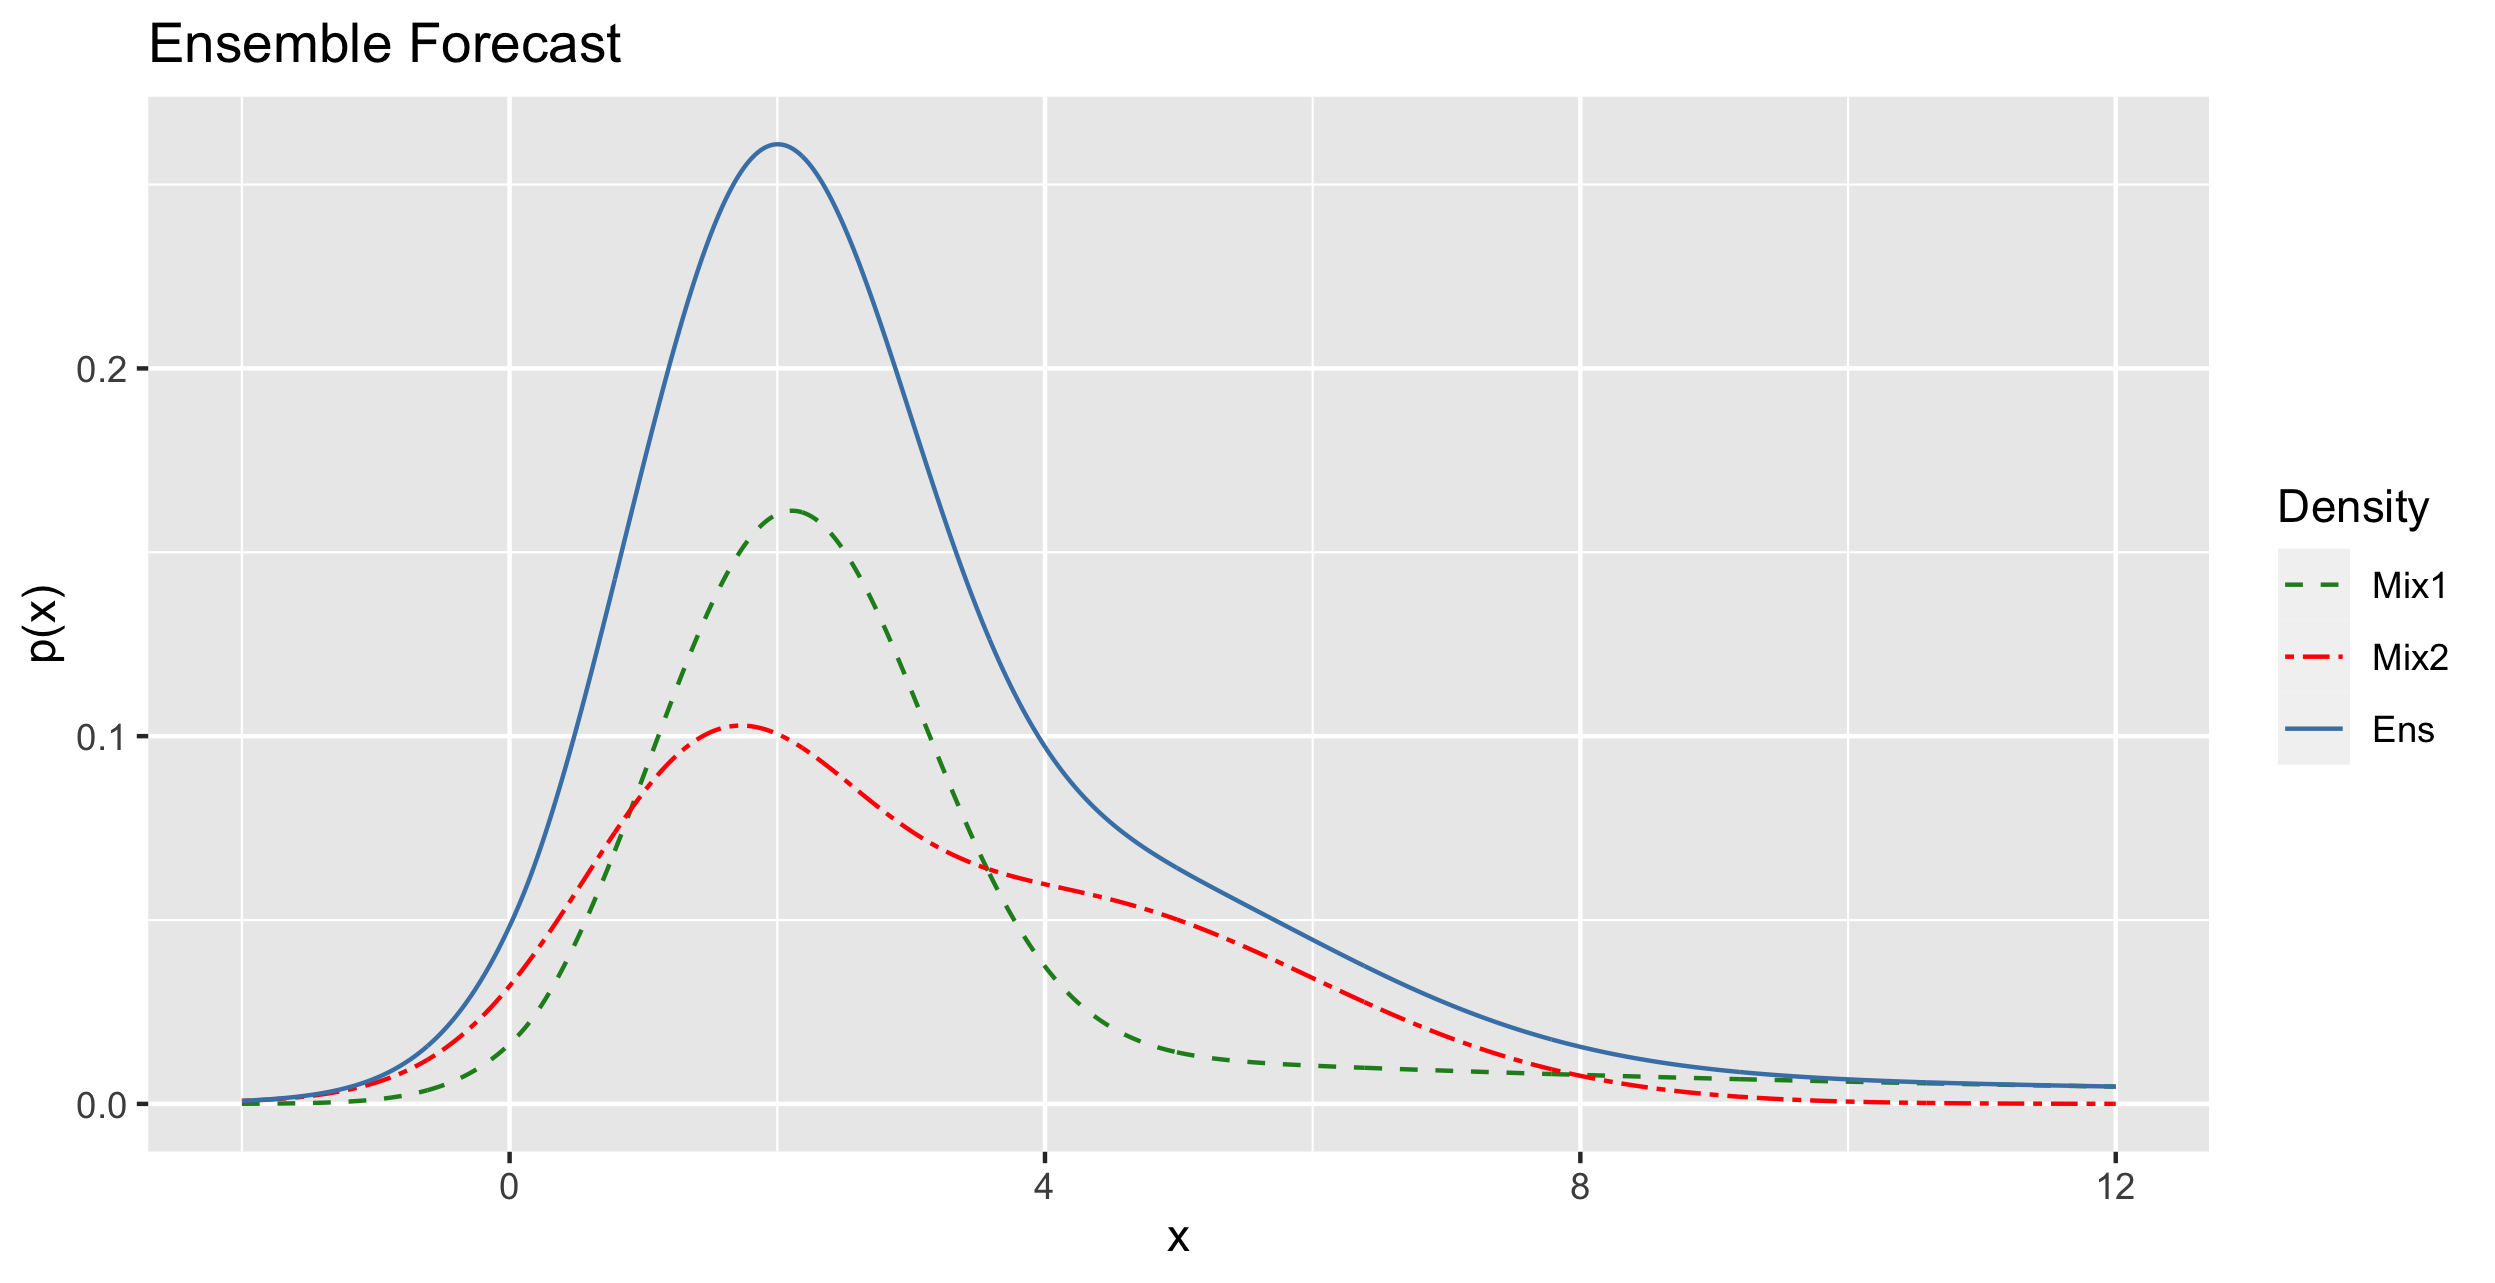
\includegraphics[scale=.15]{Images/mix_ense.png}}
\caption[Toy ensemble forecast]{Toy ensemble forecast with component mixture
distributions shown}
\label{fig:mixense}
\end{figure}

% \subsection{Mixture approximation of sample distribution}





















\section{Retrospective Analysis}
\label{section:retrostud}

For large collaborative forecast projects having already established the 
representation formats for forecasting, it may be difficult for individual
forecast teams to adjust to a discrete mixture distribution format. Exact 
methods for modeling and forecasting may not cater well to submitting a forecast
as a discrete parametric mixture distribution.

In this section we attempt to assess whether or not any forecasts from the CDC
influenza forecast competition and the COVID-19 Forecast Hub were generated from
common continuous parametric distributions. The forecasts we assess are in the 
forms of discretized bin predictions or sets of predictive intervals. In these
formats, not knowing anything about distributions or samples,  formal 
statistical methods for fitting to parametric distributions 
and assessing fit do not exist. Thus any results stated here may not be stated
in terms of statistical certainty.


\subsection{CDC Influenza like Illness}
The CDC Retrospective Forecasts project at zoltrdata.com (cite??) contains over
850,000 probabilistic influenza-like illness predictions for all combinations
of eleven regions 
in the United States and seven targets from twenty-seven different models. These
include predictions during Influenza season between October 2010 and December
2018. All predictions are in the form of discretized probability bins. 

We wanted to determine whether or not some or any of these binned forecasts were
generated from known uniform, normal, 
lognormal or gamma continuous distribution families. 
The process we followed for making such a claim was
to fit a distribution to the probabilities provided in the forecast by
minimizing

\begin{equation}
  \sum_{i=1}^K (p_i - [F(b_i; \theta) - F(b_{i-1}; \theta)])^2
  \label{eq:mds}
\end{equation}

Here $F(\cdot; \hat{\theta})$ is a CDF, $p_i$ is the reported probability for 
the $i^{th}$ bin $B_i := [b_{i-1}, b_i)$ and $K$ is the number of bins.
The fitted parameter vector $\hat{\theta}$ is the solution to 

\begin{equation}
\arg\min_{\theta}\sum_{i=1}^K (p_i - 
[F(b_i; \theta) - F(b_{i-1}; \theta)])^2
\label{eq:discfit}
\end{equation}

If a well known continuous distribution was fit to the submitted binned 
prediction
and the mean sum of squared differences (MSD) or \ref{eq:msd} fell below a 
specified cutoff value, we
considered that the binned predictions were plausibly discretized from the 
continuous distribution.


To determine what values to use as cutoffs we conducted a study where 
binned distributions were discretized from known continuous distributions, 
parameters were fit to the binned distrubtions and the MSD was calculated.

For each of uniform, truncated normal (TN), truncated lognormal (TL) and 
truncated gamma (TG) distributions the following was
done 1,000 times. A set of 131 bins with interval lengths of 
0.1 between 0 and 13.1 was constructed. 
A value $\mu$ was selected from a $Uniform(a,b)$ distribution and $\sigma$ from 
a $Uniform(.05,1.6)$ distribution. $\mu$ and $\sigma$ were taken as respectively 
the center and scale parameters of a TN distribution. 
For uniform, TL and TG family
distributions, model parameters were solved for so that $\mu$ and $\sigma$ 
were roughly the mean and standard deviation. The minimization was done using 
the \texttt{optim} function in the \texttt{R} \texttt{stats} package.
Had we accounted for the changes
in moment values from the truncation, the means and standard deviations could 
have been exactly $\mu$ and $\sigma$. But we considered the differences small 
enough that it didn't matter for our purpose.

With a known distribution, probabilities $p_i =F(b_i; \theta) - F(b_{i-1})$ were
calculated for each bin. A uniform or truncated distribution from the same
family was fit to the bins by minimizing \ref{eq:msd} with the resulting
distribution function $F(\cdot; \hat{\theta})$. From the fitted distribution
$\hat{p_i} = F(b_i; \hat{\theta}) - F(b_{i-1}; \hat{\theta})$ was computed for 
each of the 131 bins. Finally the mean sum of squared probability differences
$\frac{1}{K}\sum_{i=1}^K (\hat{p_i} - p_i)^2$ was calculated. 
Table \ref{table:bincutoffs}
below shows MSD value for which 95\% of all 1,000 MSDs fell below. Those values 
were selected as the 
cutoff values for declaring whether or not a binned distribution was discretized
from a common continuous distribution.


\begin{table}[h!]
  \centering
  \begin{tabular}{l*{6}{c}r}
  Distribution          & MSD 95\%  \\
  \hline
  Uniform               & 8.809460e-05   \\
  Truncated Normal      & 1.126683e-07  \\
  Truncated Lognormal   & 3.877829e-06  \\
  Truncated Gamma       & 1.500152e-06  \\
  \end{tabular}
  \caption[Discretized bin distribution cutoff values]{If a binned 
  distribution is fit to a parametric distribution and the MSD is smaller than
  the corresponding cutoff value listed here, we consider that binned 
  distribution to have been discretized from the fit parametric distribution.}
  \label{table:bincutoffs}
\end{table}




Of the 869,638 predictions from the CDC Retrospective Forecast project, we fit
each of Uniform, TN, TL and TG distributions to 11,715 of the individual 
predictions. The MSD between the prediction probabilities and the fit
discretized probabilities was calcuated. For each prediction, the fitted 
distribution with the lowest MSD was considered the best fit and if the MSD fell
below the corresponding cutoff value listed in \ref{table:bincutoffs} we 
considered that 
the prediction was discretized from the fit distribution. 

Of the 11,715 binned distributions fit to continuous parametric distributions,
2,502 of those fits producted MSD values below the values listed in table
\ref{table:bincutoffs}. Thus we conclude that a proportion of 0.214 of those
forecasts were generated from a common parametric distribution. The results for 
the
11,715 fit distributions, which families the binned distributions were best
fit to and whether or not the fits produce an MSD below the cutoff value, 
are seen in table \ref{table:cdcresults}. Figure \ref{fig:binparamfits} is an
example of
the best fit distributions to the same binned probability distribution.

\begin{table}[h!]
  \centering
  \begin{tabular}{l*{6}{c}r}
  Distribution Family   & Total    & Total below MSD cutoff value 
  & Proportion from parametric distribution\\
  \hline
  Uniform               & 896      & 669  & 0.747  \\
  Truncated Normal      & 3,804    & 198  & 0.052  \\
  Truncated Lognormal   & 4,501    & 1,340 & 0.289 \\
  Truncated Gamma       & 2,514    & 295   & 0.117 \\
  \end{tabular}
  \caption[CDC influenza retro analysis results]{Results for CDC influenza
  forecast retro analysis}
  \label{table:cdcresults}
\end{table}

\begin{figure}[htbp]
\centerline{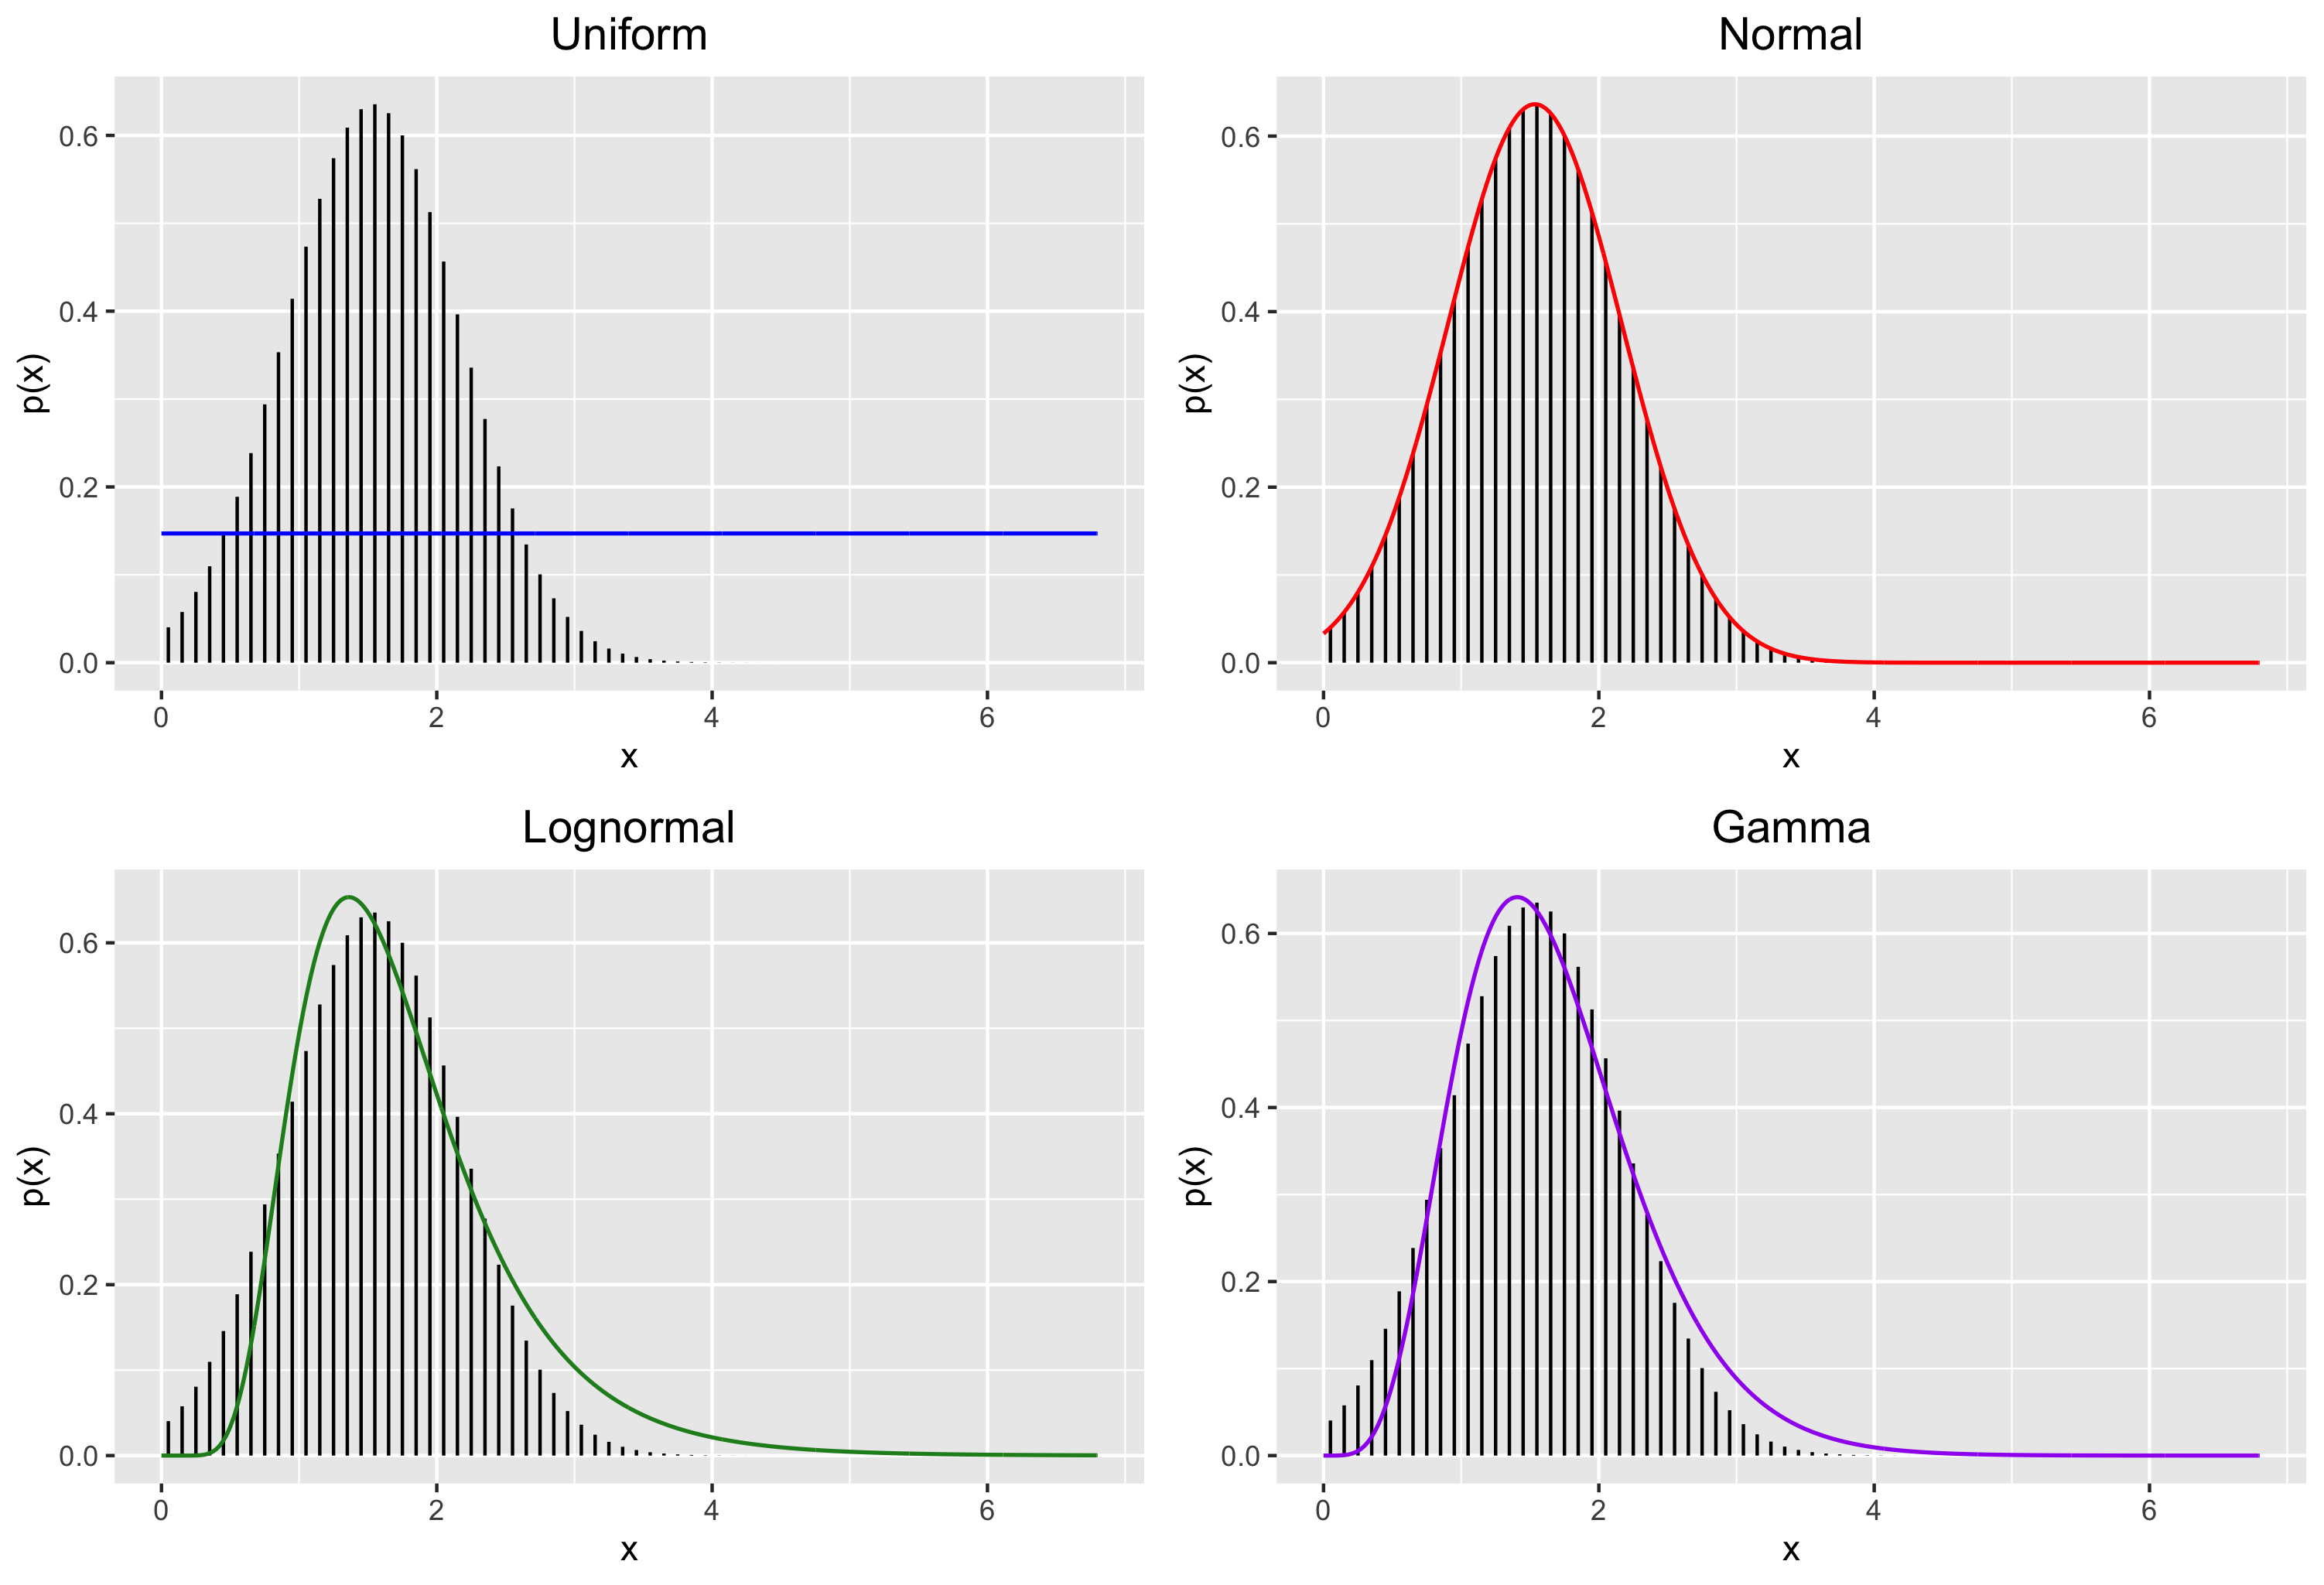
\includegraphics[scale=.15]{Images/flu_fit_17_10_3.png}}
\caption[Parametric distribution fits to binned distribution]{This figure shows
the plots of fits from each a uniform, truncated normal, truncated lognormal
and truncated gamma distributions to the same binned probability distribution.
In this case, the fit to the normal distribution produced an MSD below the 
normal cutoff value, so we conclude that the binned distribution may have been
discretized froma truncated normal.}
\label{fig:binparamfits}
\end{figure}



\subsection{COVID-19 Forecast Hub}

As of January 24, 2022 there were nearly 85,000,000 prediction distributions 
from 114 different models submitted to the COVID-19 Forecast Hub (cite??). These 
distributions covered all combinations of 3,202 municipalities (mostly counties) 
in the United States with 441 targets. The first of these forecasts was 
submitted in March of 2020 shortly after the initial outbreak of the virus in 
the US and forecasts had been received weekly since. The forecast representation
for these predictions is the quantile representation where a point estimated is
submitted along with a number of confidence intervals -three or 11 for most
targets. So the predictions typically include seven or 23 quantiles.

To assess whether or not a quantile based forecast was calculated from a well
known continuous distribution, we minimized the mean square error (MSE) between 
the CDF and the given quantiles. The estimated parameters are the 
solution to $argmin_{\theta} \sum_{i=1}^m (q_i - F(y; \theta))$ where $q_i$ is
the $i^{th}$ given quantile value and $F(y; \theta)$ is the CDF with parameter
$\theta$. This least squares estimating is a more common way to fit a model but
other methods have been presented including Bayesian Quantile Matching
\cite{nirwan2020bayesian}, step interpolation with exponential tails 
\cite{quinonero2005evaluating}
and the Method of Simulated Quantiles 
\cite{dominicy2013method}.

For each prediction used, we fit the quantiles to a uniform, normal, lognormal,
gamma and location-scale t CDF. We included the t distribution in case of any
symmetric forecasts with heavier tails than in a normal distribution.

If the MSE between a given forecast and a fit CDF fell below a certain cutoff,
we considered the quantiles as approximately coming from the fit CDF. To
determine the cutoff values, for each of the five distribution families the same
procedure was followed 1,000 times. 

A decision was randomly made on creating a quantile distribution with seven 
quantiles or 23
quantiles with probabilities 1/3 and 2/3 respectively. This was done because 
in the COVID-19 Forecast Hub certain targets require seven quantiles and others 
require 23. After that decision was made, a random value $\mu$ was drawn from
a $Uniform(2,000,\; 25,000)$ distribution and another value $\sigma$ was drawn
from a $Uniform(3, 200)$ distribution. These values were taken as the mean and
standard deviation and for each of the distribution families considered, the
proper transformations computed to find model parameters corresponding to the 
distribution. Quantile values were calculated for each quantile. When using a 
t distribution, a value for degrees of freedom was drawn from a 
$Uniform(2,35)$ distribution. A CDF
was fit by minimizing $\sum_{i=1}^m (q_i - F(y; \theta))$ over the parameter
vector $\theta$ and the MSE value $\sum_{i=1}^m (q_i - F(y; \hat{\theta}))$ was 
calculated. The MSE value for which 95\% of the 1,000 simulated distributions
fell below was considered the cutoff and is seen in table 
\ref{table:quantcutoffs}.

\begin{table}[h!]
  \centering
  \begin{tabular}{l*{6}{c}r}
  Distribution          & Mean Square Error 95\%  \\
  \hline
  Uniform               & 7.220667e-07   \\
  Normal                & 3.097645e-05  \\
  Lognormal             & 1.166775e-07  \\
  Gamma                 & 2.953370e-05  \\
  Location-scale T      & 0.4894471 \\
  \end{tabular}
  \caption[Quantile cutoff values]{If a set of quantiles
  is fit to a parametric distribution CDF and the MSE is smaller than
  the corresponding cutoff value listed here, we consider the quantiles to 
  have been calculated parametric distribution.}
  \label{table:quantcutoffs}
\end{table}


With these cutoff values selected, models were then fit to quantile forecasts
from the COVID-19 Forecasts on zoltardata.com. This was a computationally more
difficult problem than fitting distributions to the binned forecasts of the 
influenza project, so the number of predictions fit is much smaller. The 
predictions fit were selected from each of the 115 models with model weeks, 
targets and units selected randomly. In total 2,504 predictions were fit to each
of the five distributions, the MSE was calculated for each and the fit with the
lowest MSE was selected as the closest fit. If the MSE fell below the cutoff
specified above, we considered that the quantile prediction was approximately
from the same distribution as the fit distribution. Of the 2,504 fits, 99 of 
them produced an MSE value below the corresponding cutoff. Results for fits by
distribution are seen in table \ref{table:cresults}.
Figures \ref{fig:qqfits} and \ref{fig:cdffits} show the QQ plots and CDF plots
for different distribution fits to the same set of quantiles.


\begin{table}[h!]
  \centering
  \begin{tabular}{l*{6}{c}r}
  Distribution Family   & Total    & Total below MSE cutoff 
  & Proportion from parametric distribution\\
  \hline
  Uniform               & 239      & 0    & 0    \\
  Normal                & 609      & 74   & 0.122    \\
  Lognormal             & 694      & 0    & 0    \\
  Gamma                 & 597      & 0    & 0    \\
  Location-scale T      & 365      & 25   & 0.068    \\
  \end{tabular}
  \caption[COVID-19 Forecast Hub results]{Results for COVID-19 Forecast Hub
  retro analysis}
  \label{table:cresults}
\end{table}


\begin{figure}[htbp]
\centerline{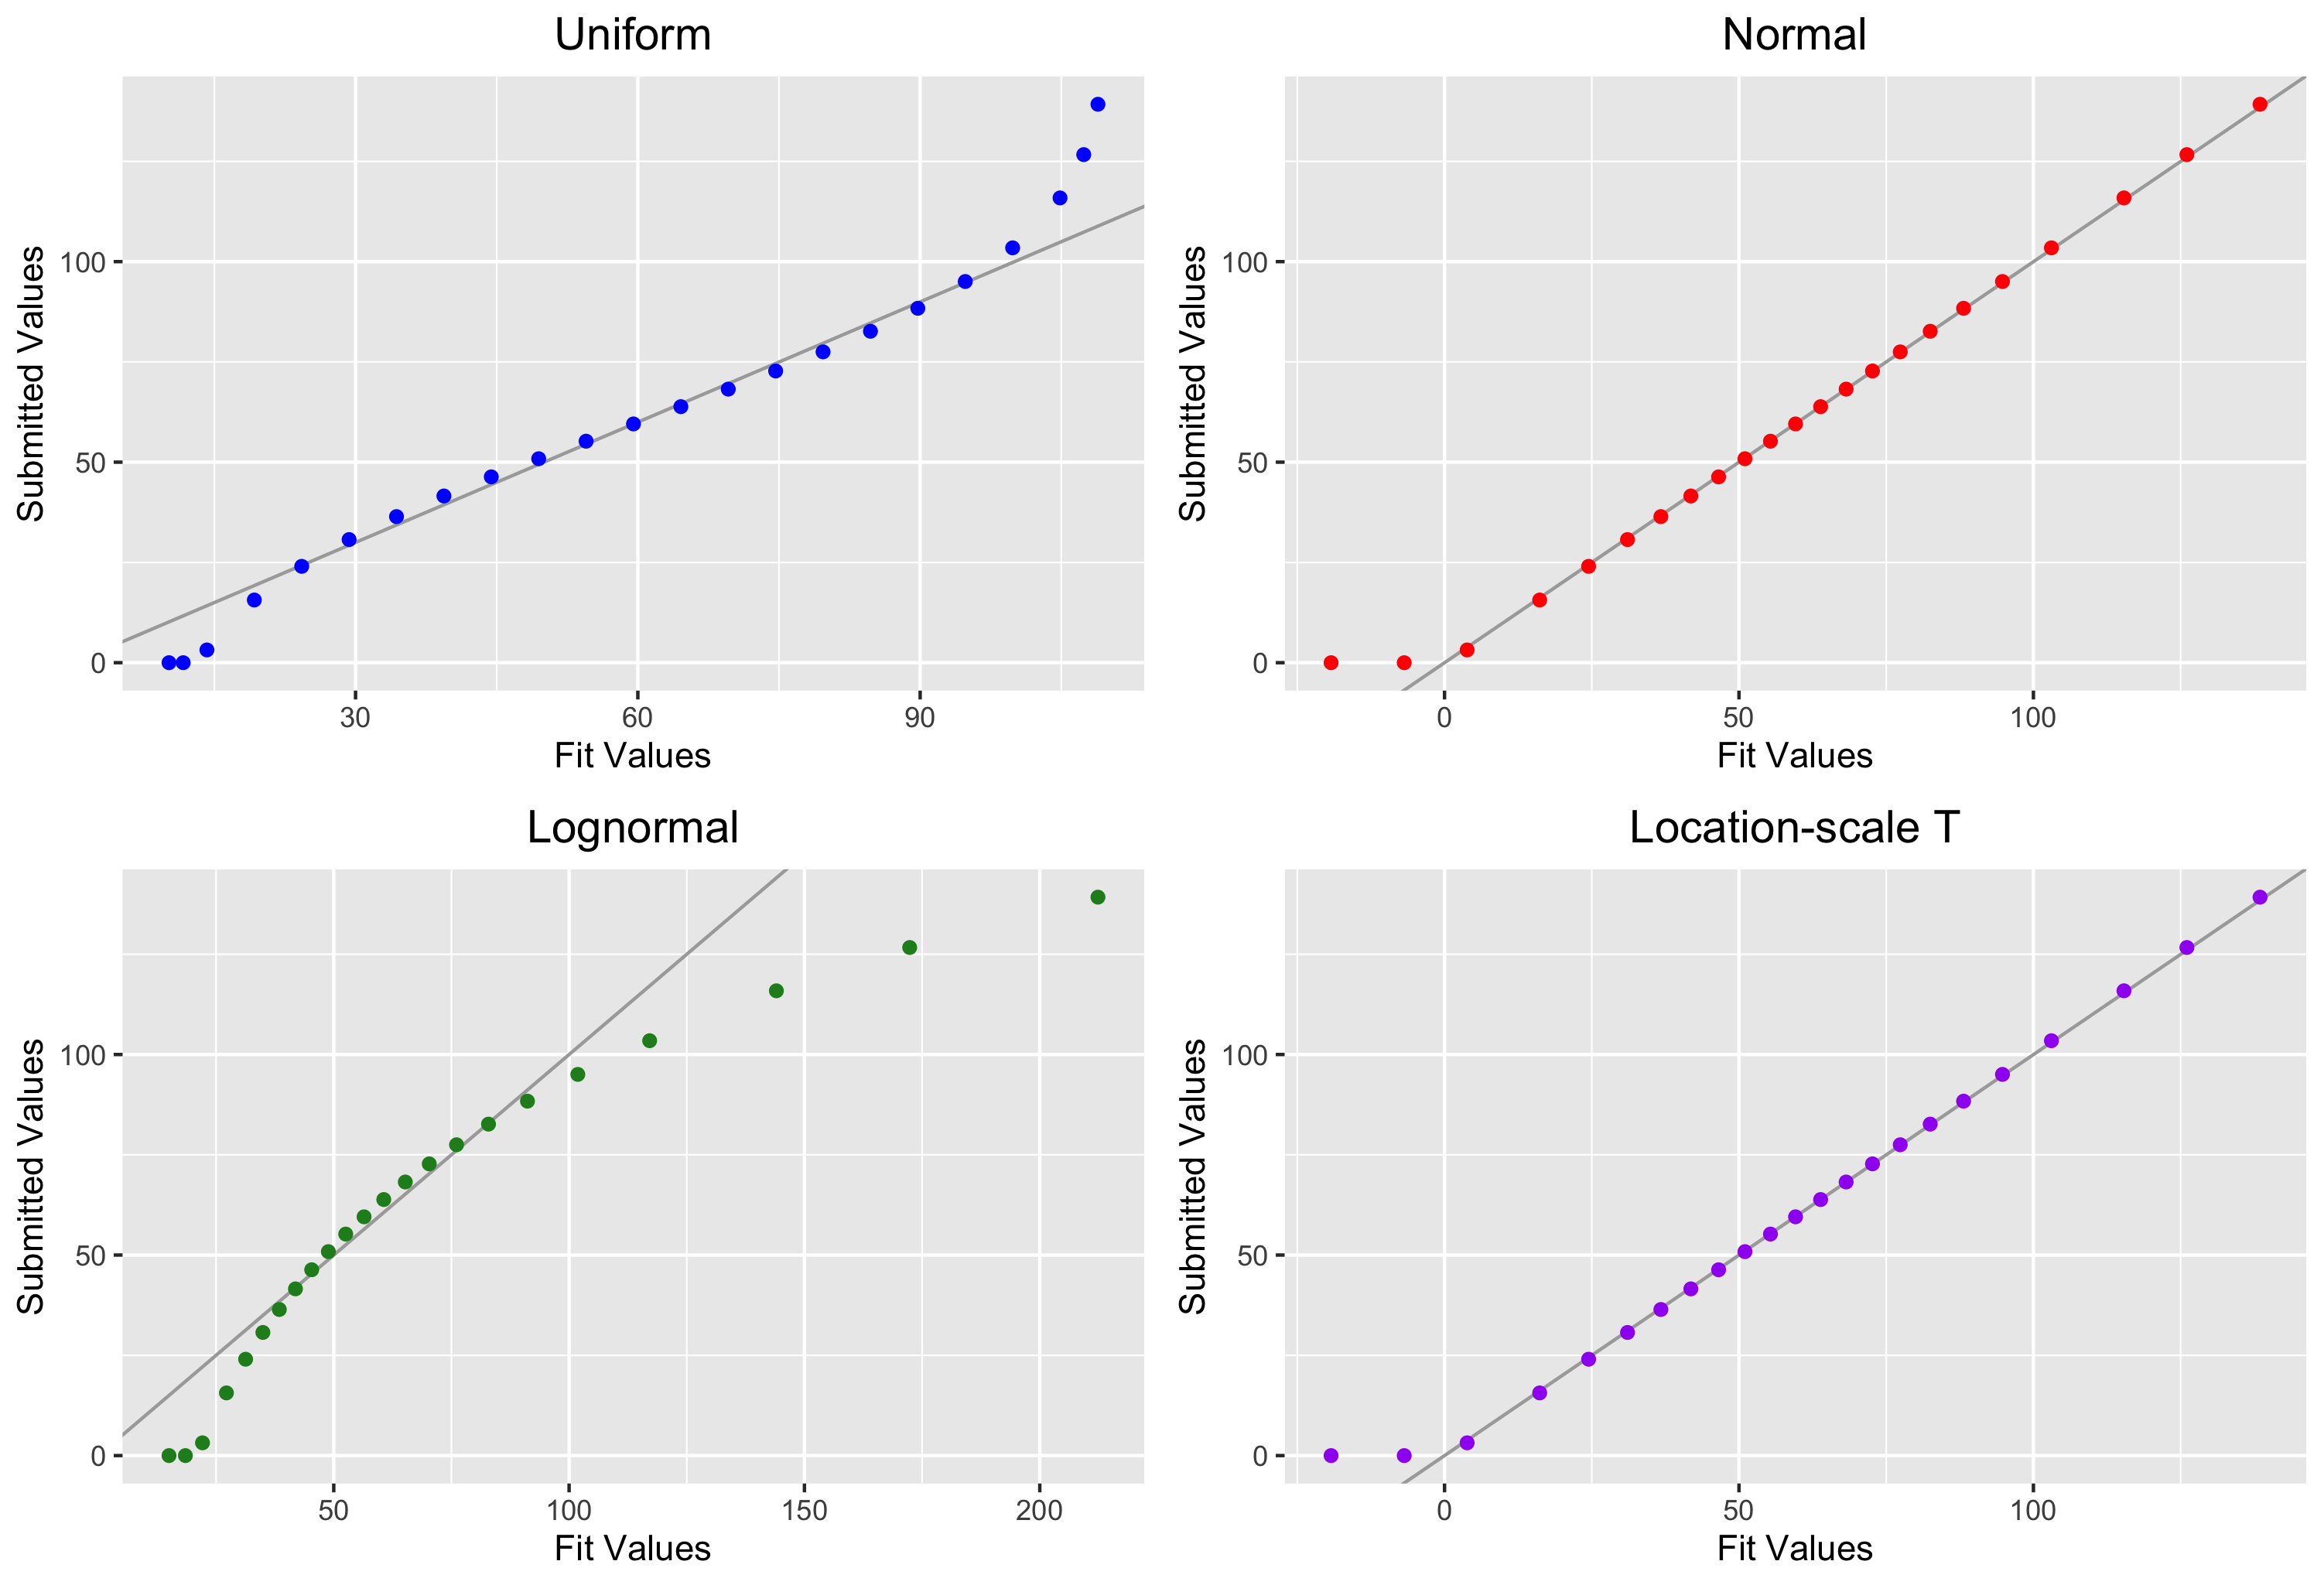
\includegraphics[scale=.15]{Images/qq_11_12_5.png}}
\caption[QQ plot for quantile fit]{This figure shows qq plots for a set of
submitted quantiles against the quantiles the continuous distribution to which
it was fit. In no case here was the MSE below the cutoff value of the 
corresponding distribution.}
\label{fig:qqfits}
\end{figure}

\begin{figure}[htbp]
\centerline{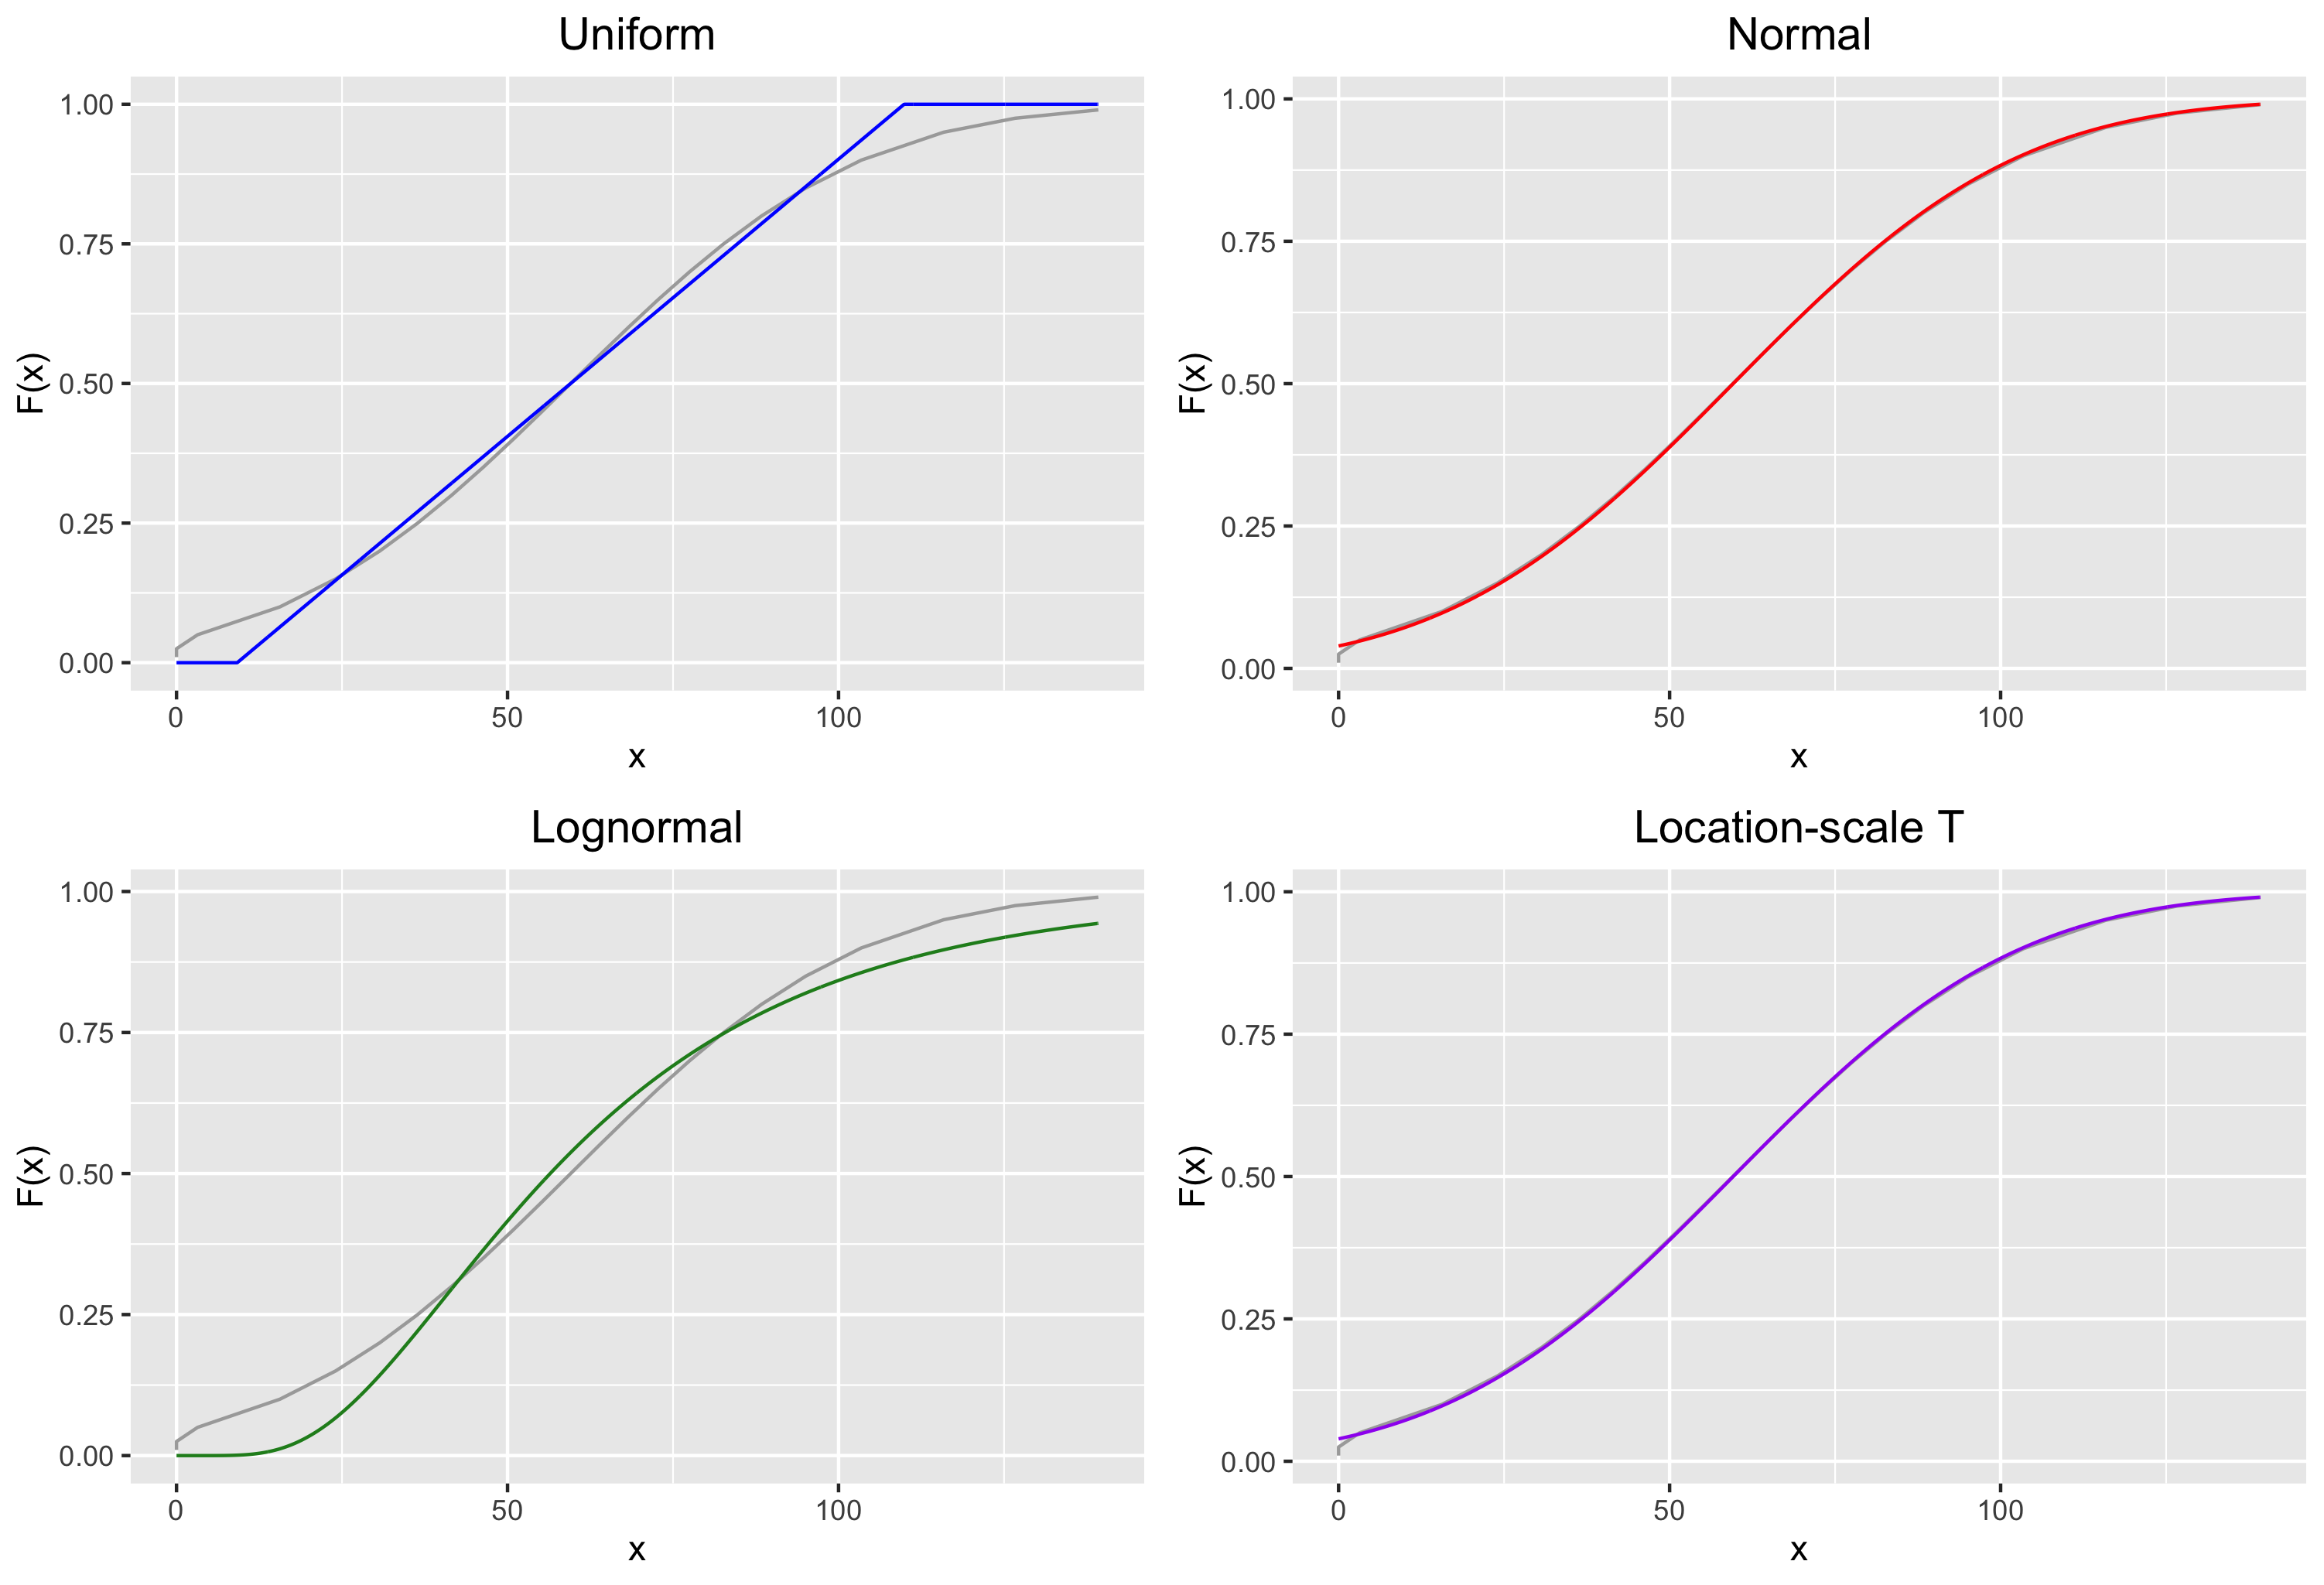
\includegraphics[scale=.15]{Images/cdf_11_12_5.png}}
\caption[CDF plot for quantile fit]{This figure shows the CDF plots for 
distributions fit to a set of quantiles. The grey line is a line of connected 
dots from the submitted quantiles and values. 
In no case here was the MSE below the cutoff value of the 
corresponding distribution.}
\label{fig:cdffits}
\end{figure}



The results in the previous two studies suggest that in some cases, forecasters
are using methods which produce simple parametric distribution forecasts. Many
likely are not. To improve upon these studies, one could fit the binned 
influenza forecasts or the COVID-19 quantile forecasts to discrete mixture 
distributions with multiple components. Forecasts that are very close to 
a mixture distribution may suggest that the forecasters already have models that
make transition to a discrete mixture distribution forecast format easy or
straightforward.














\newpage


\section{Discussion}

In this paper we have reviewed four representation types commonly used in
probabilistic 
forecasting including proper scoring, data storage and ensemble model 
construction for each type. We presented the discrete mixture distribution
representation and we argue that its use in collaborative probabilistic 
forecasting is preferable to the other representations.
In terms of model flexibility, storage and 
ensemble building it is
comparable to discretized bins and interval forecasts but also provides a 
forecast with a infinite nominal resolution. Thus we advocate its use in
future forecasting projects like those done by the CDC and COVID-19 Forecast 
Hub.

For a number of reasons, the adoption of finite mixture distributions as the
submission format may face hurdles. A collaborative forecast center, along with 
forecasters, using a 
different representation may simply not want to break from tradition. The 
implementation of new scoring and ensemble construction methods may be a 
barrier. One aspect of ensemble construction which received little attention in 
this paper is the selection of weights for components of an ensemble where each
of the components is mixture distribution. Computing requirements could become a
concern in such a problem and further research on this may provide
ideas of best methods for weight selection.

Another area of recommended research is the use of joint distributions for 
forecasting. We have only considered here probabilistic forecasting of one 
event at a time. Number of new infections in one week at one specific location
for example. This forecast is presented as a marginal distribution for that 
specific target, time and location. A joint distribution for forecasting 
multiple targets, times or locations may sometime be desirable and may require
further consideration on how joint mixture distributions could be used as a 
format in collaboration.






















% \include{Body/ch1/ch1_main}
% \include{Body/ch2/ch2_main}
% \include{Body/ch3/ch3_main}
% \include{Body/ch4/ch4_main}
% \include{Body/ch5/ch5_main}
%\include{Body/ch6/ch6_future_and_conclusions}

%\bibliographystyle{acm} % use for numbered citations along with options given in preamble. Look at the main thesis.tex file
\bibliographystyle{apa}
\bibliography{master_bib}


\section{Appendix}

The following is the code to make the \texttt{MakeDist()} function introduced 
in \ref{section:tools}.
\begin{Schunk}
\begin{Sinput}
> MakeDist <- function(distsdf){
+   
+   distdf <- distsdf[distsdf[,1] != 'Lst',]
+   tdist <- distsdf[distsdf[,1] == 'Lst',]
+   
+   fun_dist <- 
+     apply(distdf, FUN=function(x) {
+       paste('distr::',x[1], '(', 
+             ifelse(!is.na(x[2]) & (!is.na(x[3]) | !is.na(x[4])),
+                    paste(x[2],',',sep=''),
+                    ifelse(!is.na(x[2]) & is.na(x[3]) & is.na(x[4]),
+                           x[2], '')), 
+             ifelse(!is.na(x[3]) & !is.na(x[4]),
+                    paste(x[3],',',sep=''),
+                    ifelse(!is.na(x[3]) & is.na(x[4]), x[3],'')), 
+             ifelse(!is.na(x[4]),x[4],''), ')',sep='')
+     }, MARGIN = 1
+     )
+   
+   fun_tdist <- apply(tdist, FUN=function(x) {
+     paste0('distr::Td(',x[4],')*',x[3], '+', x[2])
+   }, MARGIN = 1
+   )
+   
+   dist_args <- paste(fun_dist, collapse=',',sep='')
+   tdist_args <- paste0(fun_tdist,collapse=',')
+   args <- ifelse(tdist_args!='',paste(dist_args,tdist_args,sep=','),dist_args)
+   
+   weights <- c(distdf[,5],tdist[,5])
+   mixString <- paste('distr::UnivarMixingDistribution(',
+                      args,',mixCoeff=weights)',sep='')
+   mixDist <- eval(parse(text=mixString))
+   
+   return(mixDist)
+ }
\end{Sinput}
\end{Schunk}


The following is the code used to make the function \texttt{CRPS()} used in
section \ref{section:tools}.
\begin{Schunk}
\begin{Sinput}
> crps_integrand <- function(x,dist,y) {(dist(x) - as.numeric(y <= x))^2}
> CRPS <- function(y,dist) {
+   int <- integrate(crps_integrand,-Inf,Inf,y,dist=dist)
+   return(int$value)
+ }
\end{Sinput}
\end{Schunk}

% \section{Bibliography}
% \bibliographystyle{apa}
% % \vspace{-20pt}
% \begingroup
%     \setlength{\bibsep}{13.2pt}
%     \linespread{1}\selectfont
%     \bibliography{master_bib}
% \endgroup
% \clearpage
% \pagebreak

%%%%%% bibliographies

%\clearpage
%% \nocite{*}
%\unappendixtitle
%\newpage
%% % \phantomsection
%\addcontentsline{toc}{chapter}{BIBLIOGRAPHY}
%\section*{BIBLIOGRAPHY}
%\bibliographystyle{apa}
%\vspace{-20pt}
%\begingroup
%    \setlength{\bibsep}{14.5pt}
%    \linespread{1}\selectfont
    % \bibliography{master_bib}
%\endgroup

% Renders the citations but does not show the bibliography at the end of the thesis
%\newsavebox\mytempbib
%\savebox\mytempbib{\parbox{\textwidth}{\bibliography{master_bib}}}

\clearpage
\pagebreak

%% Only within chapter appendix is allowed for Journal style writing
%% Appendix1 file from standard thesis template

\appendixtitle 
\appendix


%% Use the following two lines for single appendix
%\unappendixtitle
%\singleappendixtitle

% Please note the appendix can be removed if the thesis does not require an overall appendix

\chapter{ADDITIONAL MATERIAL} 
This is now the same as any other chapter except that
all sectioning levels below the chapter level must begin
with the *-form of a sectioning command.

\section*{More stuff}

Supplemental material.

 % Instruction for single appendix look below
%% An example second appendix from the example thesis thesis.tex.
\chapter{STATISTICAL RESULTS}

This is now the same as any other chapter except that
all sectioning levels below the chapter level must begin
with the *-form of a sectioning command.

\section*{Supplemental Statistics}

More stuff.

\end{document}

% use \isucaption{} for all captions of figures and tables, where the captions are not too long.

% Use \isucaption[]{} with the square brackets for short caption of figure or table that goes into the list of tables and list of figures, and the curly brackets can have long captions which go with the figure/ table.

% IMPORTANT NOTES
% TABLE OF CONTENTS :
% TOPIC 1:  If you need a page break follow the steps below
% step1
% check before which chapter in the table of contents you want a page break
% step 2
% go the folder "body". There open the chapter tex file that you noted needed page break in the table of contents..
% step 3
% insert  \addtocontents{toc}{\protect\newpage} before the first line i.e. before the line \chapter{RESULTS}.

%%%%%%%%%%%%%%
% use \isucaption{} for all captions of figures and tables, where the captions are not too long.

% Use \isucaption[]{} with the square brackets for short caption of figure or table that goes into the list of tables and list of figures, and the curly brackets can have long captions which go with the figure/ table.

%%%%%% Using sub figures 
% %%% In preamble include : \usepackage{subfig}
% \begin{figure}[htbp]
% 	\centering
% 	\subfloat[first caption.\label{fig:2a}]{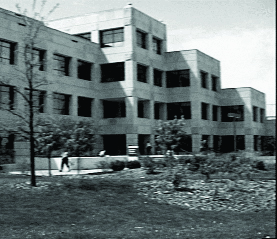
\includegraphics[width=0.2\textwidth]{Images/dc5.jpg}}\hfill
%     \subfloat[second caption.\label{fig:2b}] {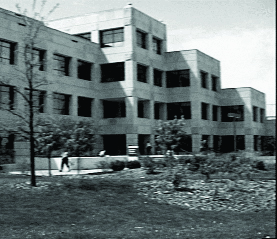
\includegraphics[width=0.2\textwidth]{Images/dc5.jpg}}\hfill
% 	\isucaption{Sub-figure test}
% 	\label{fig:subfigure-test}
% \end{figure}

% Subfloat reference: Fig \ref{fig:2a}

% Figure reference: Fig \ref{fig:subfigure-test}
